\documentclass[12pt, a4paper, oneside]{book}
% added oneside property to let the pages start equivalenty
\usepackage[utf8]{inputenc} 
\usepackage[T1]{fontenc}
\usepackage{mathpazo} 
\usepackage{algorithm}
\usepackage{algpseudocode}
\usepackage{tabularx}
\usepackage{longtable}
\usepackage{float}
\usepackage{multirow}
\usepackage{multicol}
\usepackage{pgfplots}  
\usetikzlibrary{patterns}
\usepackage{emptypage}
\usepackage{hyperref}
\usepackage{tikz}
\usepackage[square,numbers]{natbib}
\usepackage{graphicx}  
\usepackage{wrapfig} 
\usepackage{booktabs}
\usepackage{caption}
\usepackage{tfrupee}
\usepackage{tabularx}
\usepackage{xcolor}
\usepackage{listings}  
\bibliographystyle{abbrvnat}

\lstdefinelanguage{JavaScript}{
  keywords={typeof, new, true, false, catch, function, return, null, catch, switch, var, if, in, while, do, else, case, break},
  keywordstyle=\color{blue}\bfseries,
  ndkeywords={class, export, boolean, throw, implements, import, this},
  ndkeywordstyle=\color{darkgray}\bfseries,
  identifierstyle=\color{black},
  sensitive=false,
  comment=[l]{//},
  morecomment=[s]{/*}{*/},
  commentstyle=\color{purple}\ttfamily,
  stringstyle=\color{red}\ttfamily,
  morestring=[b]',
  morestring=[b]"
}

\lstset{
   language=JavaScript,
   backgroundcolor=\color{lightgray},
   extendedchars=true,
   basicstyle=\footnotesize\ttfamily,
   showstringspaces=false,
   showspaces=false,
   numbers=left,
   numberstyle=\footnotesize,
   numbersep=9pt,
   tabsize=2,
   breaklines=true,
   showtabs=false,
   captionpos=b
}

\begin{document}

\sloppy

\frontmatter

\thispagestyle{empty}

\setcounter{page}{1}

\def\thepage{\roman{page}}

\begin{center}

    \rule[0.5ex]{\linewidth}{2pt}\vspace*{-\baselineskip}\vspace*{3.2pt}
    \rule[0.5ex]{\linewidth}{2pt}

    \vspace*{3.2pt}

    {\Large\bf HumaraGhar - A Revolutionary real-estate platform.}

    \vspace*{3.2pt}

    \rule[0.5ex]{\linewidth}{2pt}\vspace*{-\baselineskip}\vspace*{3.2pt}
    \rule[0.5ex]{\linewidth}{2pt}

    \vspace{1.5cm}

    \textit{{A project report submitted in partial fulfillment of the requirements
                for the award of the degree of}}

    \vspace{1cm}

    {\bf B.Tech. in Information Technology}

    \vspace{0.5cm}

    {\bf by}

    \vspace{0.5cm}

    {\bf {Ayush Kumar}}

    \vspace{0.1cm}

    {\bf {(LIT2020024)}}

    \vspace{0.2cm}

    {\bf {Akshay Bhatnagar}}

    \vspace{0.1cm}

    {\bf {(LIT2020016)}}

    \vspace{0.1cm}

    {\bf {[Group 8]}}

    \vspace{1.1cm}

    {under the guidance of}

    \vspace{0.1cm}

    {\bf{Dr. Mainak Adhikari}}


    \vspace{1.3cm}

    
\includegraphics[height=4cm]{./Images/Logo_IIITL.png}

    {\bf\large{Indian Institute of Information Technology, Lucknow}}\\
    {\bf\fontsize{18}{20}{November 2023}}
\end{center}

\medskip

\centerline{ \copyright{} Indian Institute of Information Technology, Lucknow 2023.}

\cleardoublepage

\input certi.tex
\input acknowledge.tex
\input abstract.tex




\pagestyle{plain}

\tableofcontents

\cleardoublepage

%--------------------------------------------------------------------------------------
%	THESIS CONTENT - CHAPTERS
%--------------------------------------------------------------------------------------
\mainmatter

\setcounter{page}{1}

\def\thepage{\arabic{page}}

% Chapter 1

\chapter{Introduction}

\label{Chapter1}

\section{Background and Context}
In the evolving landscape of urban living, the challenges associated with
securing suitable accommodations transcend the boundaries of traditional
housing searches. Our endeavor to develop a room renting application stems
from the personal experiences of our team members—recent bachelor graduates
navigating their entry into professional realms in new, bustling cities.
The initial hurdle of securing affordable living spaces without an established
network of friends or acquaintances drove us to conceive a solution that
redefines the norms of housing searches.\par

\medskip

As young professionals transitioning from academic settings to bustling urban
environments, the lack of a supportive network to share the costs and experiences
of renting became a significant obstacle. This personal experience serves as the
driving force behind our initiative, inspiring us to craft a comprehensive
solution that addresses not only the financial burden but also the social and
logistical challenges associated with finding suitable accommodations and
compatible roommates.

\section{Need}
The contemporary housing market poses challenges for individuals transitioning
from academia to professional spheres, particularly in unfamiliar urban
landscapes. There exists a pressing need for an inclusive, efficient, and
user-centric platform that accommodates both solo renters and those seeking
collaborative living arrangements or compatible roommates. The absence of such
a tool creates inefficiencies and hurdles in finding affordable, compatible,
and convenient housing solutions.

\section{Problem Statement}
The challenge lies in bridging the gap between traditional housing approaches
and the modern needs of individuals seeking varied accommodation options.
The absence of a centralized platform that caters to both the individual
renter and those interested in collaborative living leads to prolonged
searches, incompatible living situations, and financial strains.

\section{Objectives}
\begin{enumerate}
      \item \textbf{Comprehensive Housing Searches:} Develop a platform that accommodates
            both individuals seeking independent rentals and those forming teams for
            collective exploration of rental spaces, ensuring inclusivity and
            convenience.
      \item \textbf{Efficient Roommate Matchmaking:} Create a robust matchmaking system
            that caters not only to those in search of compatible roommates but also to
            individuals seeking solo accommodations, ensuring tailored matches.
      \item \textbf{AI-Driven Rent Price Suggestions:} Utilize machine learning models t
            rained on diverse rent data to suggest optimal rent prices for listed
            properties, empowering users with informed pricing strategies.
      \item \textbf{Owner Dashboard \& Property Management:} Enable property owners to manage their
            listings through a dedicated dashboard, facilitating tasks like sending rent
            reminders, generating contract templates for rent agreements, and ensuring seamless
            property management.
      \item \textbf{Controlled Chat Feature:} Implement a secure and controlled chat function, allowing
            users to interact and negotiate further deals only with authorized and interested
            parties, enhancing user security and convenience.
      \item \textbf{User-Centric Design:} Prioritize user experience by delivering an intuitive
            interface that simplifies the search for accommodations or roommates,
            irrespective of the individual's preferences.
      \item \textbf{Addressing Financial and Social Barriers:} Alleviate the challenges associated
            with securing affordable living arrangements and establishing connections in
            new cities, catering to diverse housing needs.
\end{enumerate}

\section{Scope}
The project aims to develop a Next.js-based web application utilizing Supabase, a PostgreSQL-based
backend, to create a scalable, dynamic, and responsive platform. The focus lies in providing a
holistic solution catering to both individuals seeking independent rentals and those in search
of compatible roommates, fostering a sense of community and ease in the process of finding suitable
accommodations.Leveraging machine learning models, the platform will suggest rent prices for listed
properties, while a controlled chat feature will enable secure interactions between authorized users,
further enhancing the platform's utility and user experience.

% Chapter 2

\chapter{Literature Review} %chapter title

\label{Chapter2} % For referencing  use \ref{Chapter2} 

Summarizing and analyzing existing research, studies, and relevant
publications that relate to our project.

\section{Market Trends in India}
\subsection{Real Estate Market Trends}
\begin{enumerate}
      \item \textbf{Urbanization and Population Growth:} India's rapid urbanization
            continues to drive demand for housing. With a growing population
            and increasing urban migration, the need for affordable and
            accessible housing remains a significant trend.~\cite{urbanization-and-its-impact-on-housing}
      \item \textbf{Shift in Rental Preferences:} There has been a shift in preferences
            among the younger population towards rental accommodations
            due to mobility for jobs, lower commitment, and financial
            flexibility. This shift is particularly notable in metro cities
            and urban hubs.
      \item \textbf{Co-living and Co-working Spaces:} Emerging trends show a rise in
            demand for co-living spaces and co-working environments, especially
            among millennials and young professionals. These spaces offer a sense of
            community, shared amenities, and cost-effectiveness.\par
            The rise of co-living and co-working spaces is not just a trend; it's a
            significant shift in urban lifestyles. In densely populated cities like
            Mumbai, Delhi, and Bengaluru, these concepts are addressing the challenges
            of affordable housing and the need for flexible, productive workspaces.
            Moreover, co-living offers attractive returns—2-4 times higher than the
            traditional residential yield of 2-3 per cent—leading to higher investors’ i
            nterest in actively pursuing options in the market to create flexible
            co-living facilities.~\cite{investors-on-coliving}
      \item \textbf{Tech Integration in Real Estate:} Technology adoption in real estate
            has seen substantial growth. Digital platforms for property searches,
            virtual property tours, and online rent payment systems have gained
            popularity, enhancing convenience for both landlords and tenants.
      \item \textbf{Government Initiatives:} Various government initiatives like the
            Pradhan Mantri Awas Yojana (PMAY) and Smart Cities Mission aim to
            provide affordable housing and improve infrastructure, influencing the
            real estate landscape and rental market dynamics.
\end{enumerate}

\subsection{Rental Market Trends}
\begin{enumerate}
      \item \textbf{Rise in Rental Yields:} Despite fluctuations, rental yields have been stable or
            rising in certain areas, attracting investors and encouraging property owners to
            engage in the rental market.
      \item \textbf{Demand for Flexible Rentals:} There's an increasing demand for flexible rental options,
            including short-term leases and furnished accommodations, particularly from young professionals
            and students.
      \item \textbf{Emergence of PropTech Solutions:} Proptech startups are introducing innovative solutions for
            property management, tenant screening, and rent collection, streamlining processes for both landlords
            and tenants.
      \item \textbf{Localized Rental Dynamics:} Rental markets vary significantly across different cities and regions
            in India. For instance, metropolitan areas like Mumbai and Delhi exhibit different rental patterns,
            pricing structures, and demand-supply dynamics compared to tier-II or tier-III cities.
      \item \textbf{Rental Regulations and Policies:} Rental laws and regulations, such as the Rent Control Act and
            local tenancy laws, significantly impact the rental market. Understanding these regulations is crucial
            for both landlords and tenants.~\cite{public-social-rental-housing-in-india}
\end{enumerate}

\bigskip
\subsection{Recent Developments and Future Projections}
\begin{enumerate}
      \item \textbf{Post-Pandemic Impact:} The COVID-19 pandemic has influenced the rental market, causing temporary shifts
            like increased demand for spacious homes, a surge in remote work leading to altered location preferences, and a
            focus on hygiene and safety in rental spaces.
      \item \textbf{Technology and Data Analytics:} Continued integration of technology, including AI-driven property searches,
            blockchain for secure transactions, and data analytics for market predictions, is expected to redefine the rental
            landscape, making it more efficient and transparent.
      \item \textbf{Sustainability and Green Spaces:} Growing awareness of sustainability and environmental concerns is
            influencing rental choices, with preferences for eco-friendly properties and communities on the rise.
      \item \textbf{Policy Changes:} Anticipated policy changes or amendments in rental laws, especially concerning tenancy
            agreements and rent control, could significantly impact the market dynamics in the coming years.
\end{enumerate}

\section{Why we chose the PropTech sector?}
The story of proptech startups in India took shape in the mid-2000s after the entry of Info Edge-owned
99acres and Times Internet-owned Magicbricks, Quikr-owned CommonFloor and PropTiger (REA India)-owned Makaan.com.
Following this, the story revolved around Housing.com, a once-celebrated startup which then faced a series of mishaps.
In the past five years, the proptech segment has evolved manifold and has seen startups in brokerage tech led by
Square Yards, construction tech led by Infra.Market, AI, AR, VR, IoT, SaaS, and other spaces.

\clearpage
\begin{wrapfigure}{r}{0.5\textwidth}
      \centering
      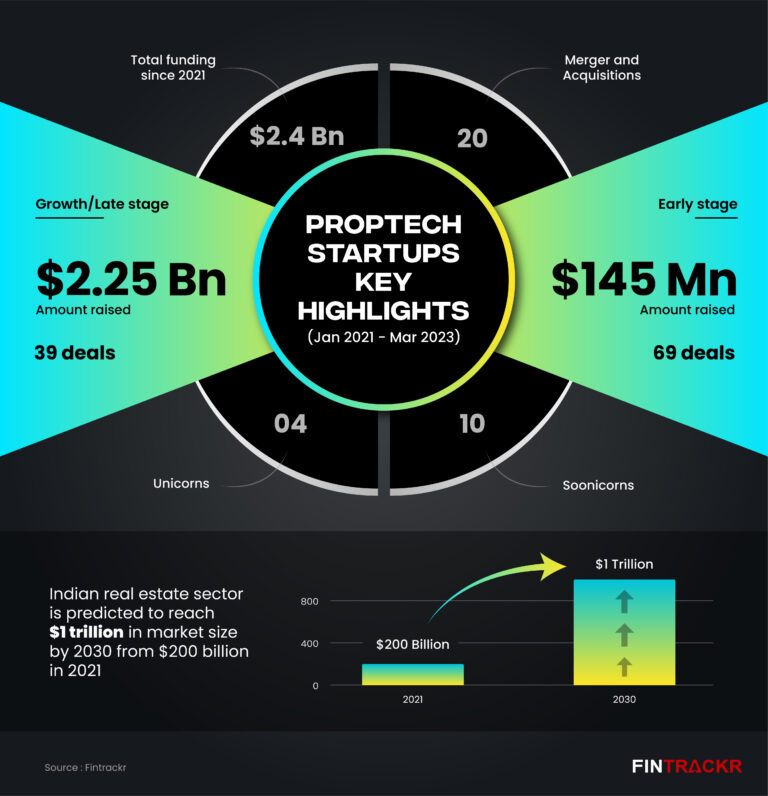
\includegraphics[width=0.48\textwidth]{Images/proptech1.jpg}
      \caption{Key Highlights}
\end{wrapfigure}

The Indian real estate sector is predicted to reach \$1 trillion in market size by 2030, up from \$200 billion in 2021,
and contribute to 13\% of the country’s GDP by 2025.  And looks like tech companies in this space have a role to play as
well. As per data compiled by Fintrackr, proptech startups have mopped up nearly \$2.4 billion between January 2021 and
March 2023. This comprises 39 growth stage companies raising \$2.25 billion and 69 early stage startups raising \$145 million.
If we take previous data, then proptech startups have managed to raise \$2.9 billion since January 2020.\par
\smallskip

Funding in proptech startups peaked in 2018 with \$1.28 billion. Even as the trend continued in 2019, the impact of lockdown
can be seen in 2020 when the fundraise plunged to less than \$500 million. This again saw a revival in 2021,
only soon to get impacted by an overall slowdown in the funding environment in 2022 and 2023. While pre-Covid era was
dominated by the likes of OYO, co-working space providers, the post-Covid period saw massive funding in construction
and building material focused startup such as Infra.Market, real estate rental startup NoBroker, home decor and interior
startups Livspace and HomeLane.~\cite{growth-of-proptech-post-covid}\par

\begin{figure}[h]
      \centering
      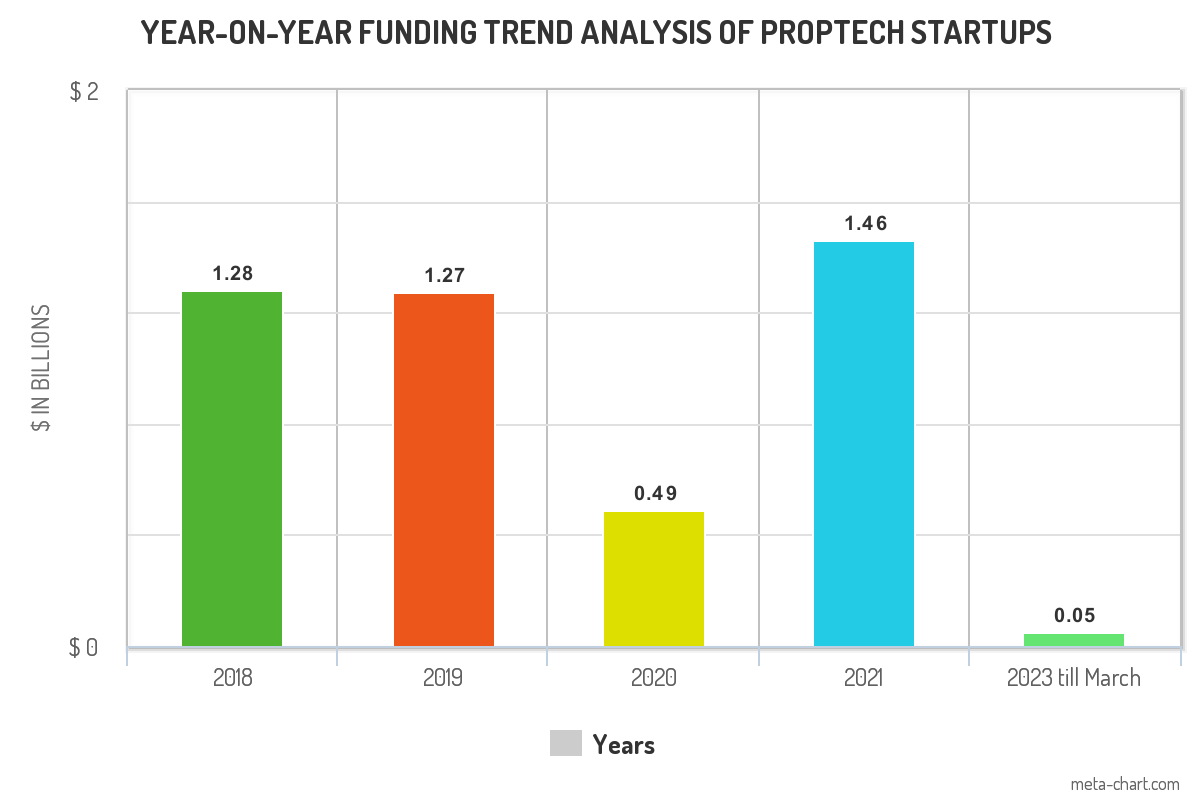
\includegraphics[width=0.7\textwidth]{Images/meta-chart.png}
      \caption{Funding trend analysis}
\end{figure}

In this section, we have highlighted top funded startups in proptech and their capital efficiency ratio based on their
financial performance in FY22.\par\medskip

\begin{table}[h]
      \centering
      \caption{Capital Efficiency of top PropTech Startups}
      \begin{tabular}{llll}
            \toprule
            Name          & Revenue(FY22)   & Overall Funding & Capital Efficiency \\
            \midrule
            IndiQube      & \rupee 6236 Cr  & \rupee 342 Cr   & 2.00               \\
            WeWork India  & \rupee 351.4 Cr & \rupee 1300 Cr  & 1.03               \\
            Awfis         & \rupee 257 Cr   & \rupee 760 Cr   & 0.50               \\
            NestAway      & \rupee 57.8 Cr  & \rupee 828 Cr   & 0.07               \\
            Stanza Living & \rupee 115 Cr   & \rupee 1672 Cr  & 0.07               \\
            NoBroker      & \rupee 116 Cr   & \rupee 2743 Cr  & 0.06               \\
            \bottomrule
      \end{tabular}
\end{table}

\begin{table}[h]
      \centering
      \caption{Top Revenue Generating Real Estate Focused Companies}
      \begin{tabularx}{\textwidth}{XX}
            \toprule
            Name         & Revenue(FY21)   \\
            \midrule
            Square Yards & \rupee 245.7 Cr \\
            Anarock      & \rupee 182 Cr   \\
            99acres      & \rupee 173.8 Cr \\
            Housing.com  & \rupee 88 Cr    \\
            PropTiger    & \rupee 50.57 Cr \\
            NoBroker     & \rupee 166.5 Cr \\
            Quikr Homes  & \rupee 60.7 Cr  \\
            MagicBricks  & \rupee 166 Cr   \\
            \bottomrule
      \end{tabularx}
\end{table}

\clearpage
\section{Co-Living \& Renting Together}

We live in a globally connected world and this has led to the real estate sector
experiencing disruption led by nomadic millennials, who are redefining the meaning
of ‘living’ and ‘working’. The concept of ‘shared economy’ has just started to
unfold in India and the days ahead look much more exciting. Unlike earlier when ‘ownership’
was fundamental to success in life, today ‘sharing’ has taken the centre stage.\par

\subsection{Framework of Analysis}
JLL Research conducted a comprehensive demand survey targeting millennials across
the top seven cities of Mumbai, Delhi NCR, Bengaluru, Hyderabad, Chennai, Kolkata
and Pune. The key objective of this assessment was to study their behavioural patterns
for owning and renting houses.\par\medskip
\begin{wrapfigure}{r}{0.5\textwidth}
      \centering
      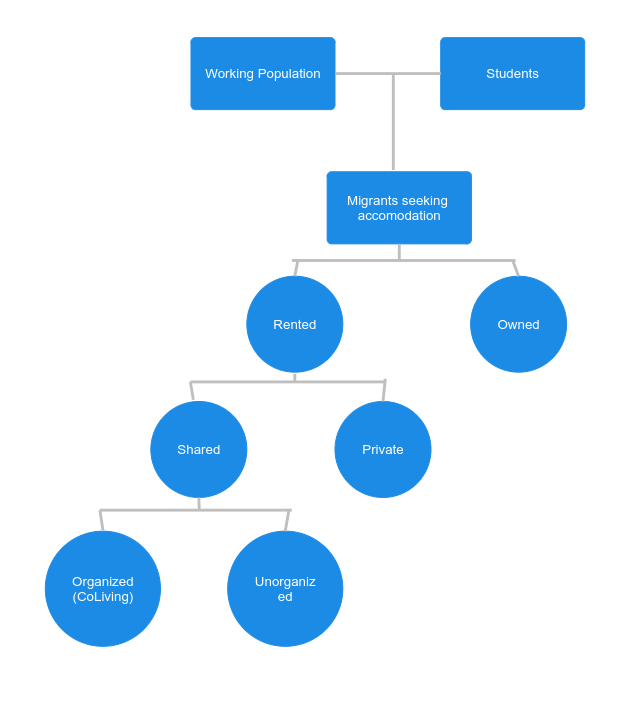
\includegraphics[width=0.48\textwidth]{Images/framework.png}
      \caption{Framework Analysis}
\end{wrapfigure}
The nomads of today are becoming a major force driving the Indian housing market—an estimated 42% of the workforce in India
constituted millennials1 in 2018 across the top seven cities in India. It is relevant to note that millennials will continue to form a major
proportion of the country’s working population, growing to nearly 41\% of the workforce in 2023.
\textbf{\textit{Nearly 40\% of India’s millennial workforce are migrants}}\par

\subsubsection{Migrant millenial workforce prefers to rent}
With millennials driving housing demand, there is a marked change in demand patterns. Gen Y has a different take on home
ownership from their parents. Earlier generations moved to the peripheral locations to fulfil their dreams of owning a home, but
millennials refuse to compromise.\par\medskip
While selecting an accommodation, connectivity to their workplace, convenience and security are the factors on top of their
decision making tree and not ownership of the property. Moreover, a migrant workforce prefers rented apartments because of the
uncertainty attached with the duration of their stay as well as cost savings in renting as against purchasing accommodation.\par\medskip
The outcome-an increased demand for rental housing.

\subsection{Owning vs Renting a house}
\noindent Home ownership has been long considered as a basis to measure financial and social security in India.
However, there has been a discernible change in the mind-set and the behaviour of the recent generations. This is attributable to the following:\par

\begin{enumerate}
      \item High cost of housing in most gateway cities and lower returns from buying a house (EMI to rent ratio is typically 2-3 times in
            most cities).
      \item Change in the nature of work - short term nature of assignments warranting higher mobility and flexibility.
      \item Delayed marriage and child rearing, less inclination to block funds and rather spend on travel, food and leisure (considered to
            be discretionary in the past).
\end{enumerate}

\begin{itemize}
      \item 93\% of the migrant respondents who were single stayed in rented accommodation across the top 7 cities
      \item 60\% said that they didn’t plan or were unsure about buying a house in the future
      \item Budget constraints and limited flexibility were cited as the key reasons for not owning a house
\end{itemize}

\clearpage
\begin{figure}[h]
      \centering
      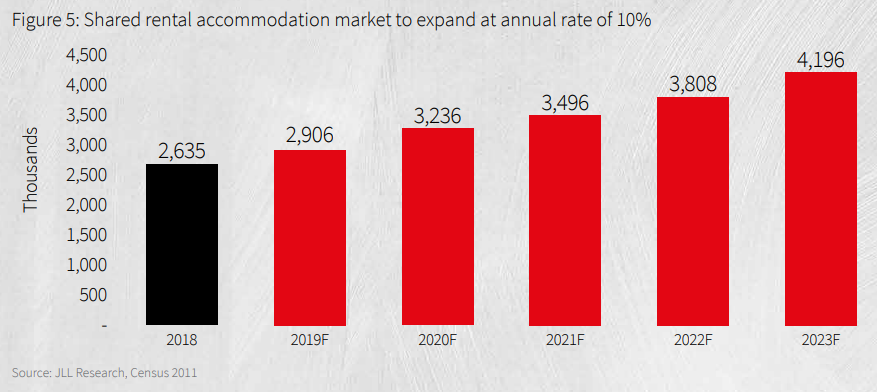
\includegraphics[width=1\textwidth]{Images/shared_market_trends.png}
      \caption{Funding trend analysis}
\end{figure}

\begin{wrapfigure}{l}{0.4\textwidth}
      \centering
      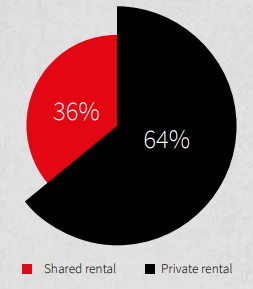
\includegraphics[width=0.35\textwidth]{Images/shared_pref.png}
      \caption{Living Preferences}
\end{wrapfigure}

Here's Why Milennials Find Shared Rental Apartments Most Vaiable:
\begin{itemize}
      \item Cities like Delhi, Pune, Hyderabad, Bengaluru, Mumbai, Chennai and Kolkata attract
            millennials for education as well as employment
      \item  Millennials consider proximity to workplace or education institute as most important while
            choosing accommodation
      \item Renting private apartment in commercial or educational hub beyond financial means of
            most millennials
      \item With housing rent typically accounting for 25-30\% of average monthly income in urban
            India, rental costs get apportioned in case of shared accommodation~\cite{coliving-reshaping-rental-housing-in-india}
\end{itemize}

% Chapter 3

\chapter{Methodology}

\label{Chapter3} % For referencing the chapter elsewhere, use \ref{Chapter3} 

\section{Development Approach}

While starting the project, we had two methods or idealogies to go by
either following a waterfall model or an agile model. The waterfall model
is a sequential design process, used in software development processes,
in which progress is seen as flowing steadily downwards (like a waterfall)
while the agile model is a practice that promotes continuous iteration of
development and testing throughout the software development lifecycle of the
project. Both of these models have their own advantages and disadvantages.\par\medskip

After careful consideration, we decided to go with a Hybrid model which is a
combination of both waterfall and agile model. Initially, we followed a Waterfall approach
for planning and designing phases of the project. After the planning and designing phase,
we tranisitioned to an agile model for the development phase of the project. This approach
helped us to have a clear idea of what we were going to do and how we were going to do it by
implementing the features in sprints, continuosly monitoring the resultings, analyzing data, and making
adjustments.

\section{Iterations and Sprints}
Our application development journey was organized into distinct sprints, each focusing on pivotal components vital to our renting platform's functionality and user experience.\par\medskip
\clearpage

\textbf{Sprint 1: Onboarding Experience}
In this sprint, our emphasis was on crafting a seamless onboarding flow. We concentrated on creating an intuitive and user-friendly registration process, ensuring users effortlessly navigate through initial setup, profile creation, and account authentication.\medskip

\textbf{Sprint 2: Dynamic Dashboard Design}
Our team dedicated this sprint to developing a dynamic and informative dashboard. Here, the focus was on designing an interface that offers users a comprehensive overview of their rented properties, team collaborations, and reminders, fostering a centralized hub for efficient property management.\medskip

\textbf{Sprint 3: Room Rental \& Roommate Finder Logic}
In this sprint, the spotlight was on formulating and implementing robust logic for room rental and roommate finder functionalities. We concentrated on refining algorithms that power property searches, match roommates based on preferences, and streamline the rental process for individual users and collaborative teams.\medskip

\textbf{Sprint 4: AI-Driven Price Prediction Model}
A critical phase, this sprint was dedicated to integrating an AI-driven price prediction model. We meticulously crafted and integrated machine learning algorithms to provide accurate rental price estimations, enhancing transparency and aiding users in making informed decisions.\medskip

\textbf{Sprint 5: Team Invitation Management}
Here, our focus shifted towards creating and implementing the logic necessary to create and manage team invitations effectively. We engineered a system that allows users to form collaborative teams seamlessly, enabling efficient property searches and shared responsibilities among team members.\medskip

\textbf{Sprint 6: Robust Chat System}
The final sprint concentrated on the development of a robust chat system. We engineered a communication platform that fosters seamless interaction between users, facilitating easy communication within collaborative teams, aiding in decision-making, and enhancing overall user engagement.\par\bigskip

These delineated sprints encapsulate the strategic breakdown of our development process, allowing us to iteratively build, test, and refine specific components of our renting application, culminating in a comprehensive and user-centric platform.

\section{Tools and Technologies}

\subsection{Programming Languages and Frameworks}

\textbf{Next.js Framework with TypeScript:}
Our renting application was built upon the Next.js framework, utilizing TypeScript for enhanced type safety and code clarity. Next.js, combined with TypeScript, empowered us to develop a robust, scalable, and statically typed application, ensuring improved code quality and developer productivity.

\medskip\noindent
\textbf{Shadcn UI Components:}
Shadcn UI components played a pivotal role in expediting the frontend development process. These pre-designed components, coupled with TypeScript support, facilitated rapid UI development, ensuring consistency and aesthetic appeal across the application.

\medskip\noindent
\textbf{React-Hook-Forms with Zod Validators:}
For efficient form management and data validation, we integrated React-Hook-Forms with Zod validators. This amalgamation, leveraging TypeScript's typing capabilities, allowed for seamless form handling, validation, and data integrity checks.

\subsection{Development Tools}
\textbf{VSCode Editor:}
Visual Studio Code (VSCode) remained our IDE of choice, offering a robust development environment with TypeScript support. Its extensive feature set, including debugging tools and TypeScript linting, facilitated efficient coding practices and collaboration among team members.

\medskip\noindent
\textbf{Git/GitHub Version Control:}
Git in conjunction with GitHub served as our version control system, allowing collaborative development and code management. TypeScript's typing features integrated seamlessly with Git, aiding in version tracking and ensuring code consistency.

\medskip\noindent
\textbf{Vercel for Deployment:}
Vercel's deployment platform, compatible with TypeScript and Next.js, streamlined our deployment process. This powerful platform facilitated quick and reliable deployment, ensuring that updates were efficiently pushed to production with TypeScript support.

\medskip\noindent
\textbf{Docker}
Docker was used to run supabase locally for running supabase-cli scripts to update database migration files.

\subsection{Database Management:}
\textbf{Supabase:}
Postgres-Based DB with Buckets for Data and Image Storage;
Supabase, integrated with TypeScript for seamless data handling, functioned as our primary database solution. The PostgreSQL-based database, coupled with TypeScript's typing features, provided a secure and scalable infrastructure for storing application data and images through Supabase buckets.

\section{Development Process}

This section will summarize the development process, including how we approached the problems technically.

\subsection{Setup}

The project was initialized using create-next-app with the supabase template.\medskip
\begin{lstlisting}[language=bash]
    npx create-next-app -e with-supabase
\end{lstlisting}

\subsubsection{Cookie-based Auth}
We are using Cookie-based Auth in our web application. The Next.js Auth Helpers package configures Supabase Auth to store the user's session in a cookie, rather than localStorage. This makes it available across the client and server of the App Router - Client Components, Server Components, Server Actions, Route Handlers and Middleware. The session is automatically sent along with any requests to Supabase.\smallskip

\begin{lstlisting}[language=bash, caption={Installing Auth Helpers}]
npm install @supabase/auth-helpers-nextjs @supabase/supabase-js
\end{lstlisting}
\noindent
We are then declaring environment variables in .env.local file with following environment variables:
\begin{lstlisting}[caption={.env.local}]
    NEXT_PUBLIC_SUPABASE_URL=your-supabase-url
    NEXT_PUBLIC_SUPABASE_ANON_KEY=your-supabase-anon-key
\end{lstlisting}

The Next.js Auth Helpers are configured to use the server-side auth flow to sign in users
into the application. For this we had to setup a Code Exchange route, to exchange an auth
code for the user's session, which is set as a cookie for future requests made to Supabase.

We created a callback route handler that performs this exchange at app/api/auth/callback/route.js:

\begin{lstlisting}[language=javascript, caption={Callback Route Handler}]
import { createRouteHandlerClient } from '@supabase/auth-helpers-nextjs'
import { cookies } from 'next/headers'
import { NextResponse } from 'next/server'

export async function GET(request) {
  const requestUrl = new URL(request.url)
  const code = requestUrl.searchParams.get('code')

  if (code) {
    const cookieStore = cookies()
    const supabase = createRouteHandlerClient({ cookies: () => cookieStore })
    await supabase.auth.exchangeCodeForSession(code)
  }


  // URL to redirect to after sign in process completes
  return NextResponse.redirect(requestUrl.origin)
}
\end{lstlisting}
\clearpage
Part of inviting users to our application was having a attractive UI. We achieved this
through discussing over design language and then finalising over shadcn's collection for our UI components. Shadcn-ui contains re-usable components built using Radix UI and Tailwind CSS.

\subsubsection{Dark Mode Support}
We are using next-themes package to support dark mode in our application. This package provides a useTheme hook that allows us to access the current theme and toggleTheme function to toggle between light and dark mode. We are using this hook to toggle between light and dark mode in our application.

\begin{lstlisting}[language=bash, caption={Installing next-themes}]
    npm install next-themes    
\end{lstlisting}

\noindent Creating a theme provider\par\medskip\noindent
components/theme-provider.tsx

\begin{lstlisting}[language=javascript, caption={Theme Provider}]
"use client"

import * as React from "react"
import { ThemeProvider as NextThemesProvider } from "next-themes"
import { type ThemeProviderProps } from "next-themes/dist/types"
    
export function ThemeProvider({ children, ...props }: ThemeProviderProps) {
    return <NextThemesProvider {...props}>{children}</NextThemesProvider>
}
    
\end{lstlisting}

The created theme-provider is added to the root layout and linked with tailwind-css config file to achieve the proper result.

\clearpage
\subsection{Database Structure and Functionality}

\begin{figure}[h]
    \centering
    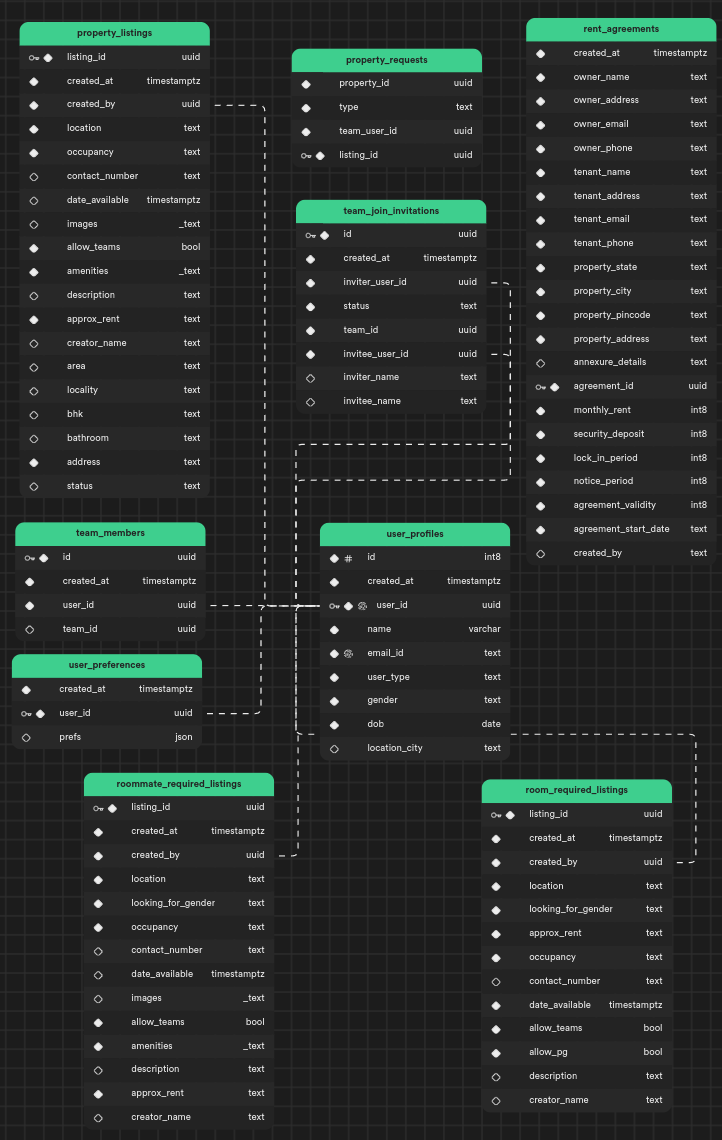
\includegraphics[width=0.7\textwidth]{Images/schema_visualizer.png}
    \caption{Funding trend analysis}
\end{figure}
This image describes the database structure of our application. We have used supabase's database and storage buckets to store our data. We have used supabase's auth to authenticate users and supabase's storage buckets to store images and other files.
\clearpage

\subsubsection{Why Supabase and PostgreSQL?}

\noindent\textbf{Utilizing Row-Level Security (RLS) Policies}
\par\smallskip\noindent One of the key features that drew us to Supabase is its implementation of Row-Level Security (RLS) policies. RLS policies enable fine-grained control over data access within the database by restricting users' access to specific rows based on defined security policies.

In our room renting application, RLS policies play a pivotal role in ensuring data security and privacy. They allow us to enforce access control mechanisms at the row level, granting users access only to the data relevant to their interactions and permissions. For instance, RLS policies dictate that users can view and interact with property listings, roommate preferences, or matchmaking data only within the scope of their authorized permissions, enhancing data confidentiality and integrity.

\par\medskip
\noindent\textbf{Triggers in PostgreSQL}
\par\smallskip\noindent PostgreSQL's robust support for triggers serves as a pivotal element in automating various processes within the database. Triggers enable the execution of predefined actions in response to specific database events, ensuring streamlined and automated workflows.

In our application, triggers play a pivotal role in orchestrating interactions between users and property listings, facilitating personalized recommendations, and triggering roommate matchmaking processes. For instance, when a user expresses interest in a property or updates their preferences, triggers activate functions that analyze compatibility, recommend suitable listings, or initiate matchmaking processes.

\par\medskip
\noindent\textbf{PL/pgSQL Functions for Automation}
\par\smallskip\noindent The integration of PL/pgSQL functions within PostgreSQL further amplifies the automation capabilities of our database. PL/pgSQL, a procedural language extension for PostgreSQL, allows the creation of custom functions to automate complex database operations.

These functions empower our system to automate tasks such as automatically moving members to correct teams after they accept or decline an invite request.

\clearpage
\subsubsection{Team Invitation Management}

Users can browser other users who have signed up for teams and filter them based on the their preferences, the preferences were already
stored during onboarding and are used to calculate a score for each user. The score is calculated by comparing the user's preferences with the
preferences of the user who is searching for a roommate.\par

We are mainly taking advantage of two tables in our schema for this purpose, team\_members and team\_join\_invitations. The team\_members table
contains mapping of users to teams and the team\_join\_invitations table contains list of all the invitations sent to users to join a team, with a column
having the status of the invite as "waiting", "accepted" or "rejected".\par
\medskip
\noindent We have a postgres trigger in place watching over the value of status and it is triggered when the value of status changes from "waiting" to "accepted".

\begin{lstlisting}[language=sql]
CREATE TRIGGER "on_team_invitation_accepted_trigger"
AFTER
UPDATE ON "public"."team_join_invitations" FOR EACH ROW
    WHEN (
    (
        ("old"."status" <> "new"."status")
        AND (
        "new"."status" = 'accepted'::"text"
        )
    )
) EXECUTE FUNCTION "public"."handle_add_team_member_after_invitation_accepted"();
\end{lstlisting}

\noindent The trigger calls a function handle\_add\_team\_member\_after\_invitation\_accepted which adds the user to the team and updates the values in team\_members table.
\begin{lstlisting}[language=sql]
create function "public"."handle_add_team_member_after_invitation_accepted" () returns "trigger" language "plpgsql" security definer as $$BEGIN
UPDATE team_members
SET team_id = NEW.team_id
WHERE user_id = NEW.invitee_user_id;
    
IF NOT FOUND THEN
INSERT INTO team_members(user_id, team_id)
VALUES (
    NEW.invitee_user_id,
    NEW.team_id
    );
END IF;
RETURN NEW;
END;
$$;
\end{lstlisting}

\noindent The changes are then reflected in the application and the user is added to the team.

\subsection{Rent Agreement Generation}

The implementation of a multi-step form using the useMultiStepForm React hook stands as a cornerstone in our room renting application, specifically facilitating the seamless input of data required for generating rent agreements in PDF format. This client-side process employs the react-pdf package for PDF generation and utilizes file-saver to enable users to download the finalized agreement.\par\medskip

\noindent
\textbf{Functionality of the Mutli-Step Form}\par\medskip\noindent
The useMultiStepForm hook was custom-built to guide users through a structured sequence of input fields necessary for creating a comprehensive rent agreement. Each step of the form collects specific information, such as:

\begin{itemize}
    \item Agreement details
    \item Tenant details
    \item Owner details
    \item Property details
    \item Additional details
\end{itemize}
\noindent
The structured nature of the multi-step form ensures that users provide all necessary information required to generate a legally binding rent agreement.

\medskip
\noindent
\textbf{Rent Agreement Download}\par\medskip\noindent
Upon completion of the multi-step form, the entered data is compiled and processed client-side using the react-pdf package. This package dynamically generates a PDF document based on the collected input, encapsulating the terms and clauses specified in the rent agreement.\par\medskip

Subsequently, the file-saver library is utilized to enable users to download the generated rent agreement PDF directly from the client-side interface, providing a convenient and immediate access method for users.

\medskip
\noindent
\textbf{Status of Digital Agreements in Indian Law}\par\medskip\noindent
In India, the status of digital agreements is governed by the Information Technology Act, 2000, and the Indian Contract Act, 1872. These legal frameworks recognize electronic documents and digital signatures as valid and enforceable, provided they comply with specific requirements, including:

\begin{itemize}
    \item Authentication of electronic records
    \item Ensuring the integrity of the information
    \item Obtaining consent from involved parties
\end{itemize}
Digital agreements, including electronically signed rent agreements, hold legal validity if they adhere to these stipulations outlined in Indian law.

\subsection{AI-Driven Price Prediction Model}

\subsubsection{Context}
Housing in India varies from palaces of erstwhile maharajas to modern apartment buildings in big cities to tiny huts in far-flung villages. There has been tremendous growth in India's housing sector as incomes have risen. The Human Rights Measurement Initiative finds that India is doing 60.9\% of what should be possible at its level of income for the right to housing.\par
\medskip
Renting, also known as hiring or letting, is an agreement where a payment is made for the temporary use of a good, service, or property owned by another. A gross lease is when the tenant pays a flat rental amount and the landlord pays for all property charges regularly incurred by the ownership. Renting can be an example of the sharing economy.

\clearpage
\subsubsection{Data Glossary}
\begin{itemize}
    \item \textbf{BHK:} Number of Bedrooms, Hall and Kitchen
    \item \textbf{Rent:} Price of Houses/Apartments/Flats.
    \item \textbf{Size:} Size of the House/Apartment/Flat in Square Feet.
    \item \textbf{Floor:} Floor Number of the House/Apartment/Flat
    \item \textbf{Area Type:} Type of the Area (e.g. Super built-up Area, Built-up Area, Carpet Area)
    \item \textbf{Area Locally:} Locality of the House/Apartment/Flat
    \item \textbf{City:} City in which the House/Apartment/Flat is located
    \item \textbf{Furnishing Status:} Furnishing Status of the House/Apartment/Flat (e.g. Fully Furnished, Semi-Furnished, Unfurnished)
    \item \textbf{Tenant Type:} Type of Tenant (e.g. Family, Bachelor, Company Lease, etc.)
    \item \textbf{Bathroom:} Number of Bathrooms in the House/Apartment/Flat
    \item \textbf{Point of Contact:} Contact Number of the Owner of the House/Apartment/Flat
\end{itemize}

\bigskip
\subsubsection{Data Analysis and Visualization}
\textbf{Pairplot of data}\par\bigskip\noindent

\begin{lstlisting}[language=python]
    sns.pairplot(rent_data,height=2)
    plt.show()
\end{lstlisting}

\clearpage

\begin{figure}[h]
    \centering
    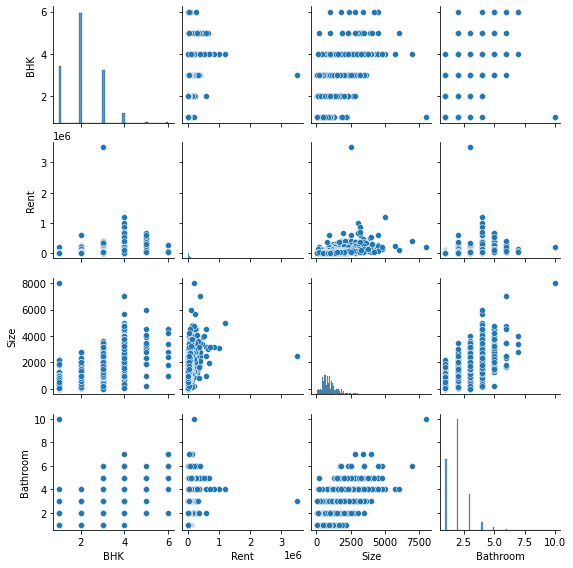
\includegraphics[width=0.7\textwidth]{Images/pairplot.png}
    \caption{Pairplot of data}
\end{figure}

A univariate and bivariate analysis was done to flush out outliers.~\cite{house-rent-prediction-model}\par\medskip

\noindent
\textbf{Rent (Our Target Variable)}
\begin{lstlisting}[language=python]
    fig = px.histogram(rent_data,x='Rent',color_discrete_sequence = px.colors.qualitative.Set3, title="Rent Prices Distribution Histogram")
    fig.show()
    fig = px.box(rent_data, x="Rent", title='Boxplot for Rent Prices')
    fig.show()
\end{lstlisting}

\clearpage
\begin{figure}[h]
    \centering
    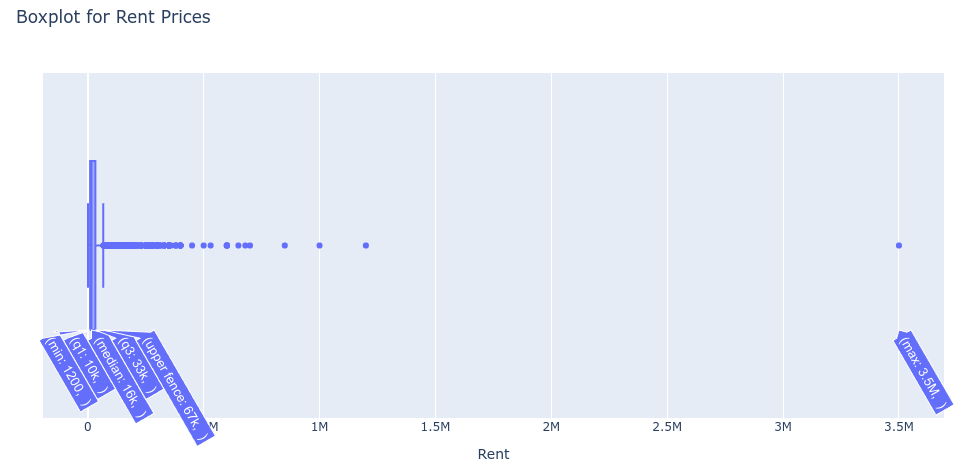
\includegraphics[width=0.7\textwidth]{Images/boxplotrent.png}
\end{figure}

\noindent\textbf{Observations:}
There is one outlier so far out of the inter-quantile range.
\medskip
\noindent\textbf{Actions:}
To remove outlier, as it may affect our assumptions about other variables and analysis

\begin{lstlisting}[language=python]
    print(np.where(rent_data['Rent']>2000000))
\end{lstlisting}

\noindent\textbf{Observations:}
Outlier's position is at 1837th position in a dataframe.
\medskip
\noindent\textbf{Deleting the outlier}
\begin{lstlisting}[language=python]
    rent_data.drop([1837], axis=0, inplace=True)

    fig = px.box(rent_data, x="Rent",title='Boxplot for Rent Prices')
    fig.show()
\end{lstlisting}

\noindent\textbf{BHK}
\begin{lstlisting}[language=python]
    rent_data['BHK'].value_counts()rent_data['BHK'].value_counts()
\end{lstlisting}


\begin{lstlisting}[language=python]
    sns.set_style('whitegrid')
    fig,axes = plt.subplots(figsize=(12,8))
    colors = ['#87ace8','#e3784d', '#6ecc64','#b644e3','#eb7c87', '#EAE509']
    
    ax = sns.countplot(x='BHK',data=rent_data, palette=['#e3784d','#87ace8', '#6ecc64','#b644e3','#eb7c87','#EAE509'])
    for container in ax.containers:
        ax.bar_label(container)
    plt.title('Frequency of different number of BHKs present in Houses available for Rent',fontsize=15)
    plt.show()
    
    fig = px.pie(rent_data, names='BHK', height=700, width= 700, color_discrete_sequence=px.colors.sequential.deep, title='Pie Chart for different number of BHKs present in Houses available for Rent')
    fig.update_traces(textfont_size=15)
    fig.show()
\end{lstlisting}

\begin{figure}[h]
    \centering
    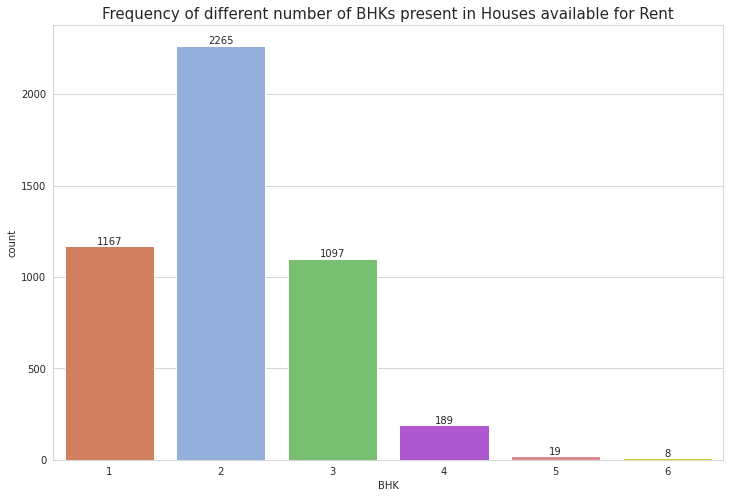
\includegraphics[width=0.7\textwidth]{Images/bhkfreq.png}
\end{figure}

\noindent\textbf{Observations:}
House with 2 Bathrooms are most common for the houses put up on rent. Houses with 7 and 10 bathroom quite seems inappropriate and not much of use.
\medskip

\noindent\textbf{City}
\begin{lstlisting}[language=python]
    rent_data['City'].value_counts()
\end{lstlisting}


\begin{lstlisting}[language=python]
    sns.set_style('whitegrid')
    fig,axes = plt.subplots(figsize=(12,8))
    colors = ['#87ace8','#e3784d', '#6ecc64','#b644e3','#eb7c87', '#EAE509']
    
    ax = sns.countplot(x='City',data=rent_data, palette=['#EAE509','#87ace8', '#6ecc64','#eb7c87','#e3784d','#b644e3'])
    for container in ax.containers:
        ax.bar_label(container)
    plt.title('City wise Houses available for Rent',fontsize=15)
    plt.show()
    
    fig = px.pie(rent_data, names='City', height=700, width= 700, color_discrete_sequence=px.colors.sequential.deep, title='Pie Chart for Houses available for Rent in different cities')
    fig.update_traces(textfont_size=15)
    fig.show()
\end{lstlisting}

\begin{figure}[h]
    \centering
    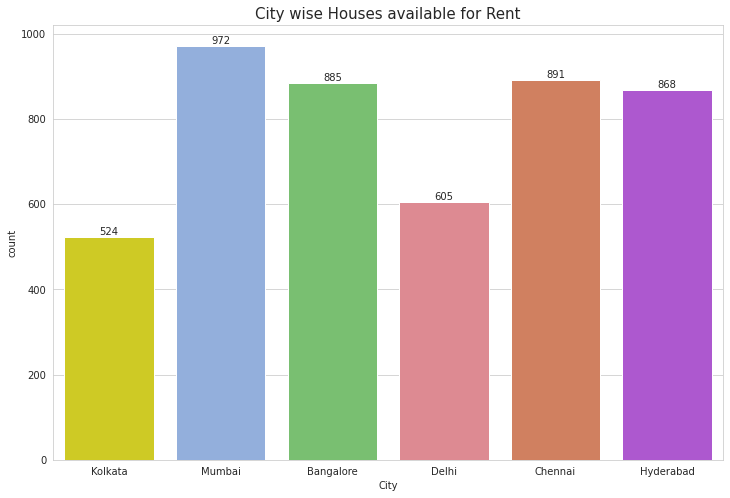
\includegraphics[width=0.7\textwidth]{Images/citygraph.png}
\end{figure}

\noindent\textbf{Observations:}
Mumbai, followed by Chennai and Hyderad has most number of rented houses, seems like there is very high demand considering the job corporates and other factors.
\medskip

\noindent\textbf{Liner Regression}\par
\noindent\medskip
A Linear Regression model was used to predict the prices in our application.\par
\medskip
The most extensively used modelling technique is linear regression, which assumes a linear connection between a dependent variable (Y) and an independent variable (X). It employs a regression line, also known as a best-fit line. The linear connection is defined as Y = c+m*X + e, where ‘c’ denotes the intercept, ‘m’ denotes the slope of the line, and ‘e’ is the error term.\par
\medskip
The linear regression model can be simple (with only one dependent and one independent variable) or complex (with numerous dependent and independent variables) (with one dependent variable and more than one independent variable).

\medskip
\noindent\textbf{Training the model}\par\medskip
\noindent\medskip
The model was trained using the following code:

\begin{lstlisting}[language=python]
    def predict_price(location,Size,bath,BHK):
    loc_index = np.where(X.columns == location)[0][0]
    
    x = np.zeros(len(X.columns))
    x[0]= BHK
    x[1]= Size
    x[2]= bath 
    if loc_index >=0:
        x[loc_index]=1
    
    return lr_clf.predict([x])[0]
\end{lstlisting}

using linear regression model we created a function to predict rental prices
\begin{lstlisting}[language=python]
    import pickle
    with open('rent_prices_model.pickle','wb') as f:
    pickle.dump(lr_clf,f)
\end{lstlisting}

\medskip
\noindent
After training our model we exported model as a pickel file so that we can load it in our flask server
we also exported json file containing all available locations in our model

\begin{lstlisting}[language=python]
    import json
    import pickle
    import numpy as np
    import sklearn
     
    __locations = None
    __data_columns = None
    __model = None
     
    def get_estimated_price(location,sqft,bath,bhk):
        try:
            loc_index = __data_columns.index(location.lower())
        except:
            loc_index =-1
        x= np.zeros(len(__data_columns))
        x[0]= bhk
        x[1]= sqft
        x[2]= bath
        if loc_index >=0:
            x[loc_index]=1
     
        return round(__model.predict([x])[0],2)
     
    def get_location_name():
        return __locations
     
    def load_saved_artifacts():
        print("loading saved artifacts... start")
        global __data_columns
        global __locations
     
        with open("./artifacts/columns.json",'r') as f:
           __data_columns= json.load(f)['data_columns']
           __locations = __data_columns[3:]
     
        global __model
        with open("./artifacts/rent_prices_model_1.pickle",'rb') as f:
            __model = pickle.load(f)
        print("loading saved artifacts...done")
     
    if __name__ == '__main__':
        load_saved_artifacts()
        print(get_location_name())
        print(get_estimated_price('Adambakkam',1200,2,3))
     
\end{lstlisting}

% Chapter Template

\chapter{Simulation and Results} % Main chapter title

\label{Chapter4}
In this section we will going over all the part of our app one by one simulating a user’s
workflow.\par\noindent

\section{Login and Signup}
The landing page is the
first page that the user will see when he/she opens the app. The landing page is shown in\par
\begin{figure}[h]
    \centering
    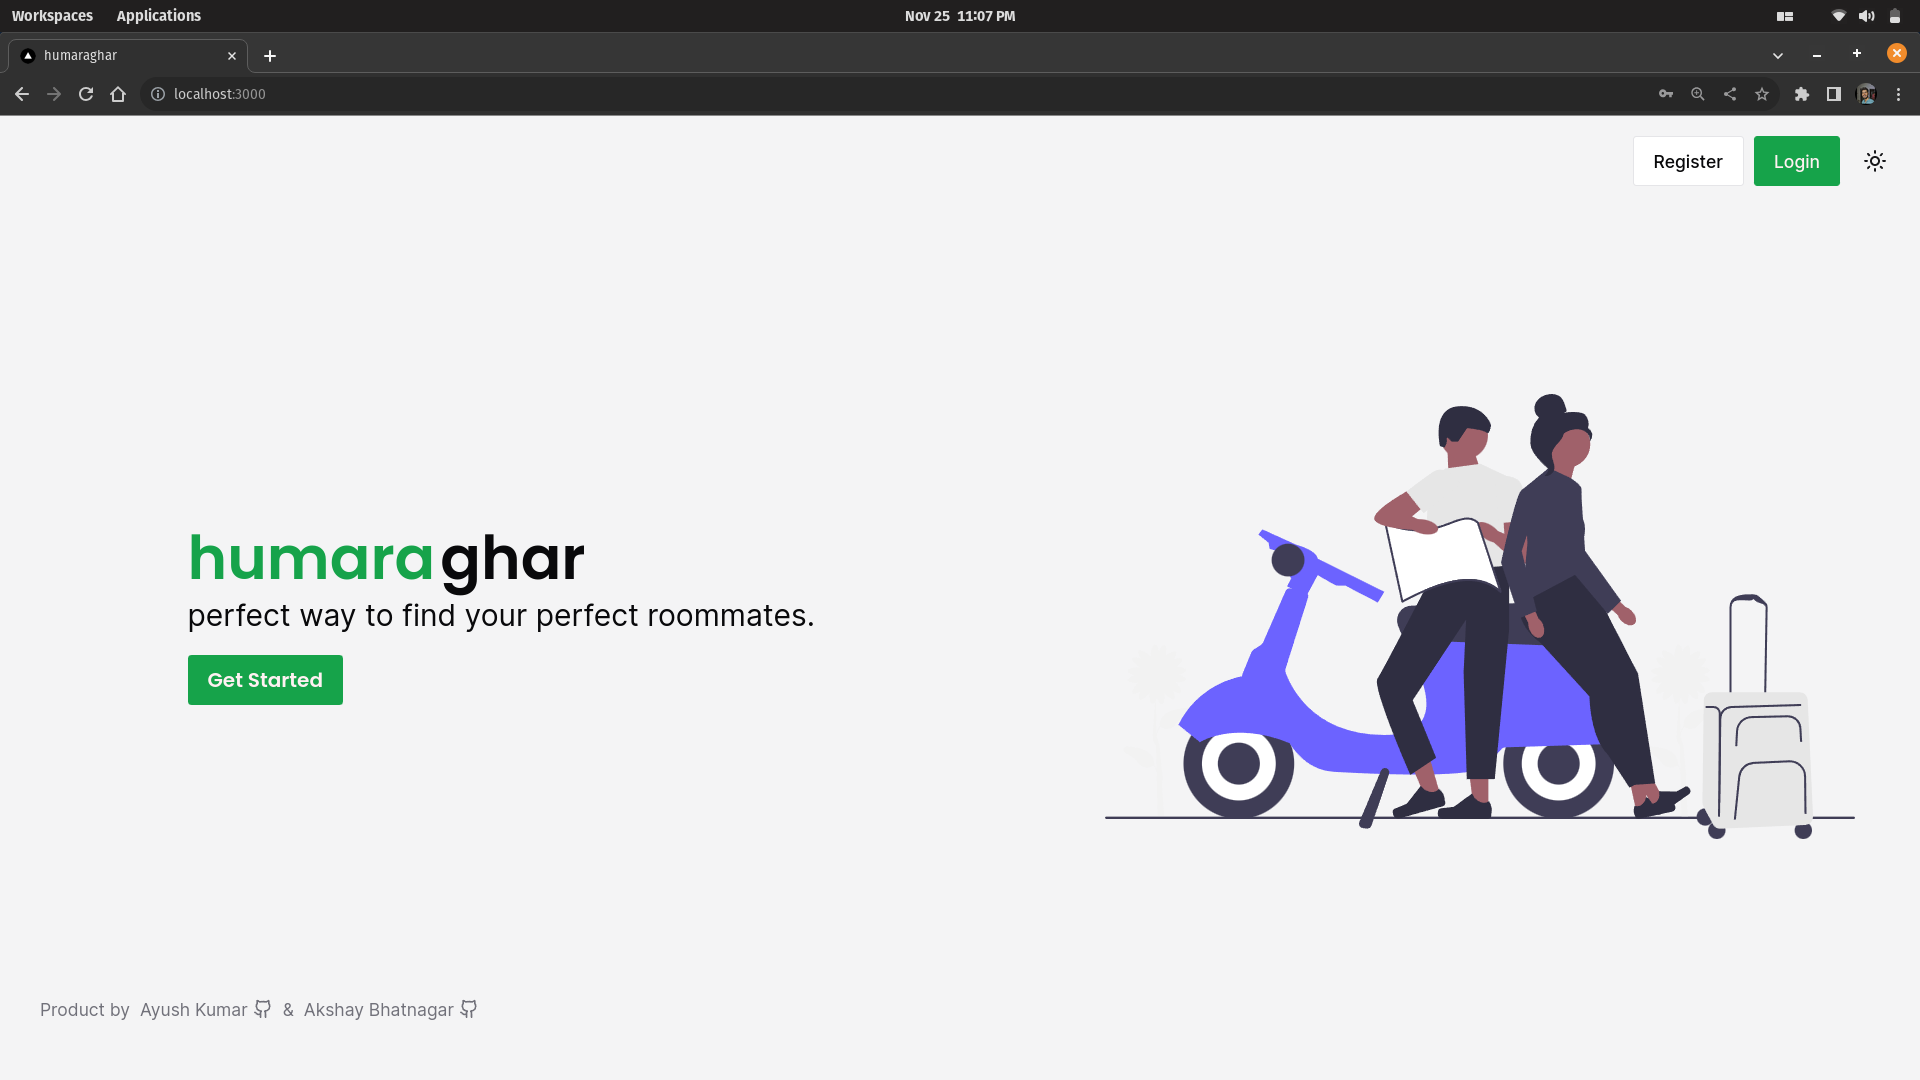
\includegraphics[width=1\textwidth]{Images/screenshots/landing.png}
    \caption{Landing Page}
\end{figure}
\noindent
The landing page contains a button that will take the user to the sign-up/login page or directly to the dashboard if
already signed in.\par\noindent

\clearpage
The sign-up/login page is shown in \par
\begin{figure}[h]
    \centering
    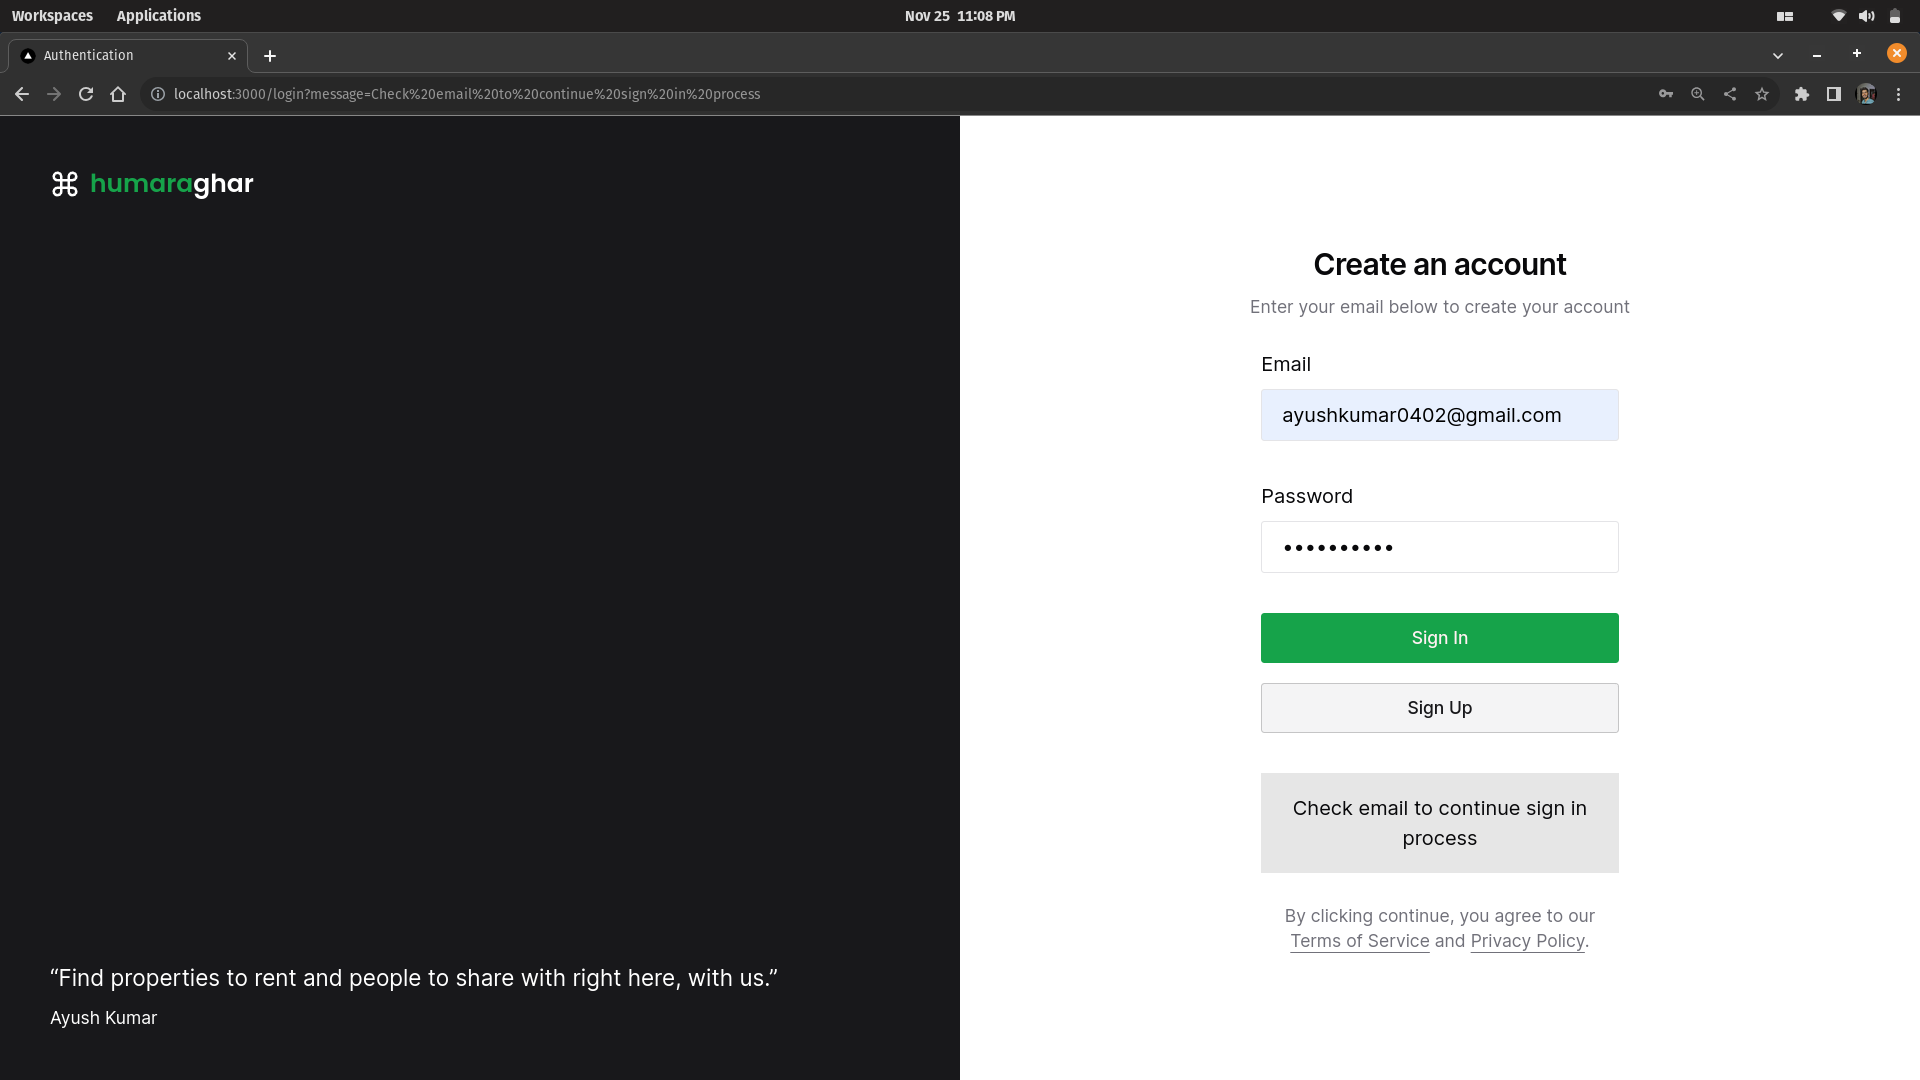
\includegraphics[width=0.9\textwidth]{Images/screenshots/signup.png}
    \caption{Login Page}
\end{figure}

On entering the correct details, a verification mail will be sent to the user’s email address. The user will have to
verify his/her email address to be able to login. The verification mail is shown in \par
\begin{figure}[h]
    \centering
    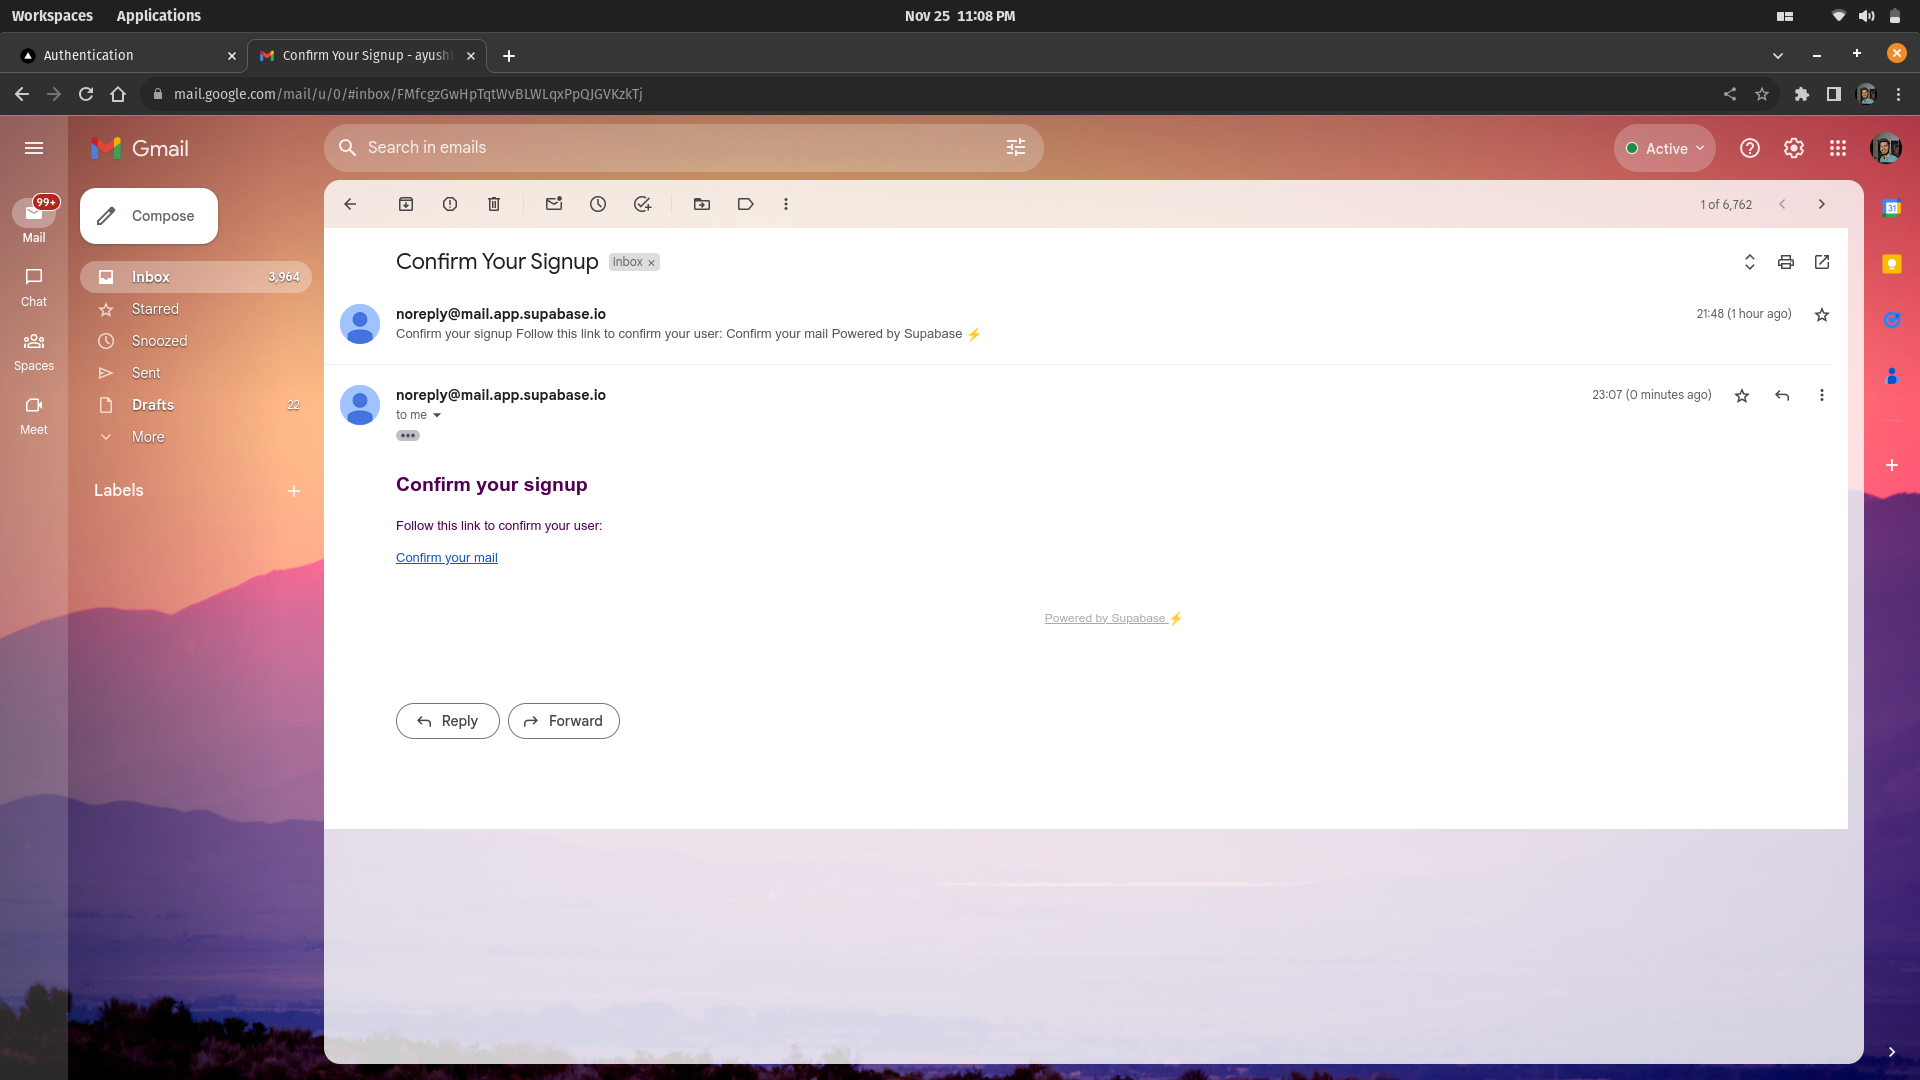
\includegraphics[width=0.8\textwidth]{Images/screenshots/mail.png}
    \caption{Verification Mail}
\end{figure}
\clearpage

\section{Onboarding Flow}
The onboarding flow contains forms containing user's data. The user will have to fill the forms to be able to use the
app. The first section of onboarding process aims to collect basic information about the user:

\begin{figure}[h]
    \centering
    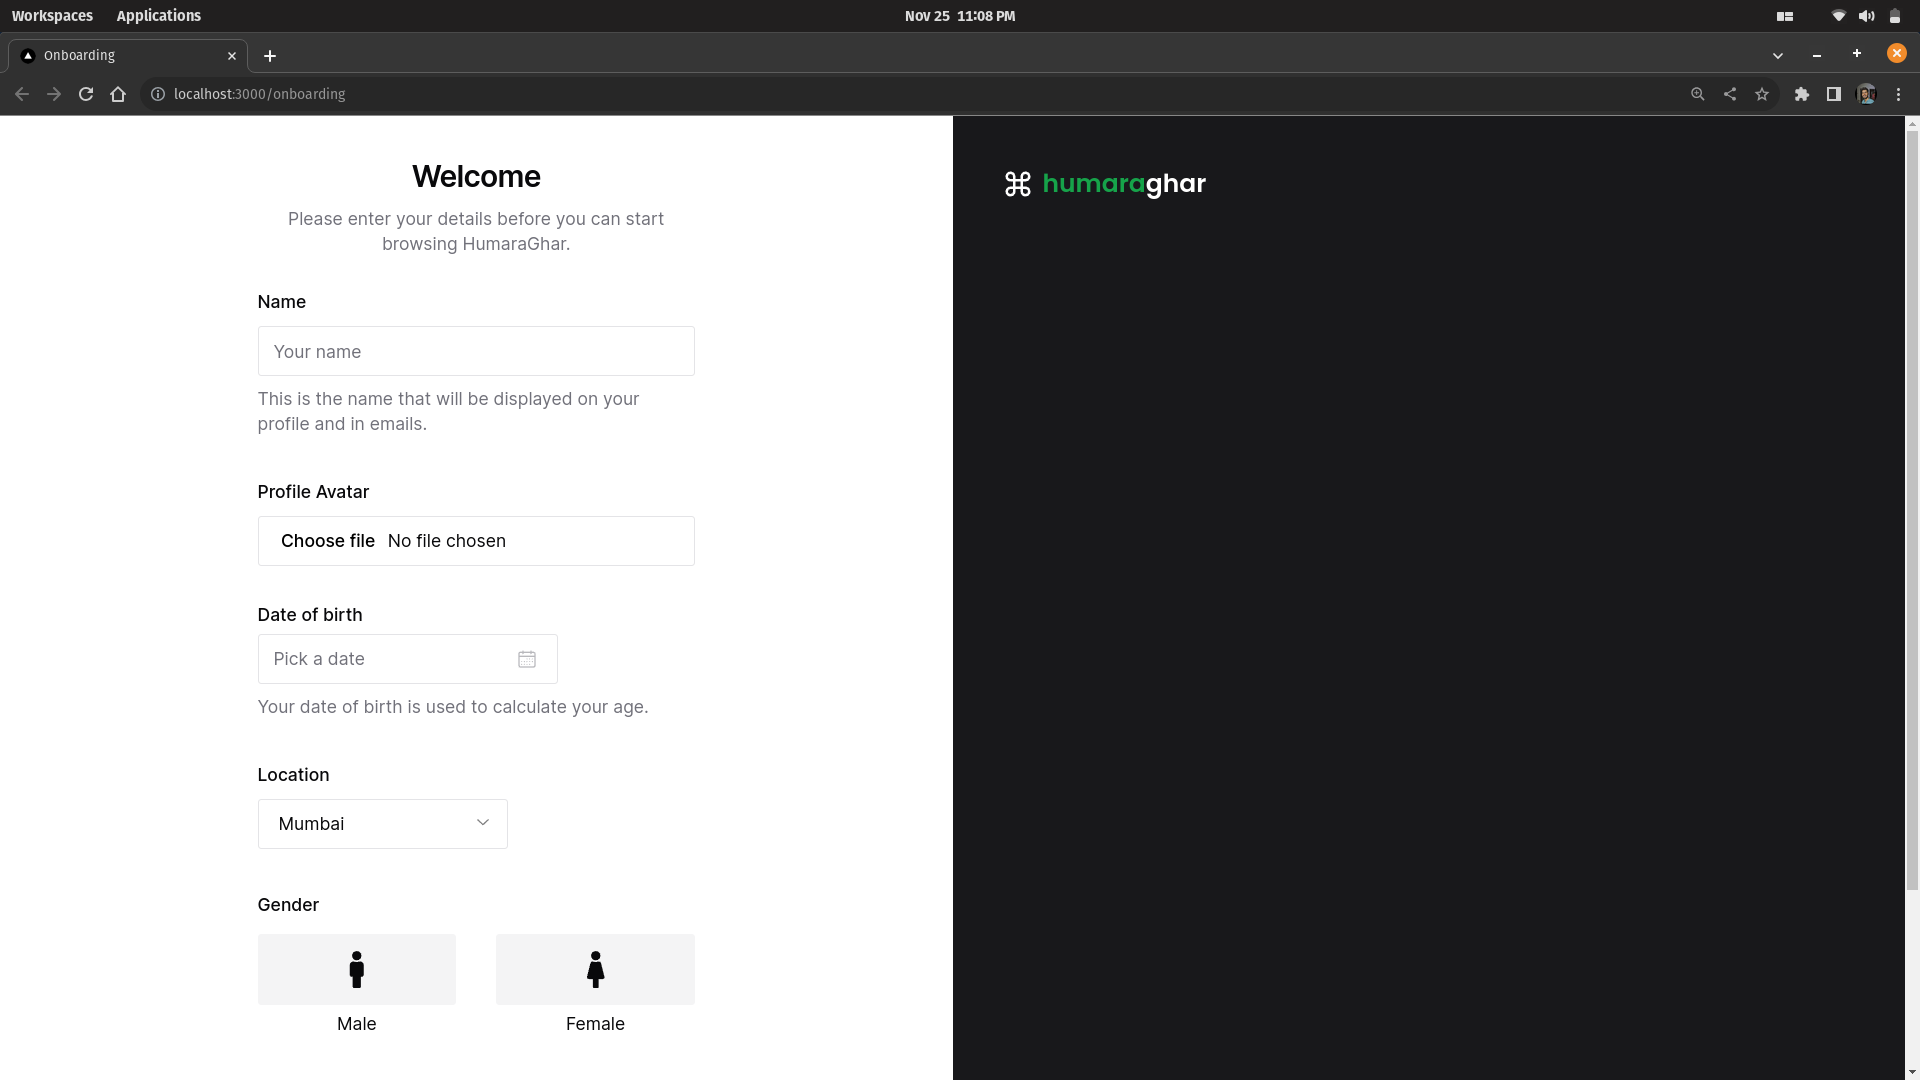
\includegraphics[width=0.8\textwidth]{Images/screenshots/onboarding.png}
    \caption{Onboarding Page 1}
\end{figure}

\par\noindent
The second section of onboarding process aims to collect information about the user's roommate preferences in case
he/she wants to share their room with someone else. The user can skip this section if he/she wants to live alone.
This data will be used to calculate match-score between users.\par
\begin{figure}[h]
    \centering
    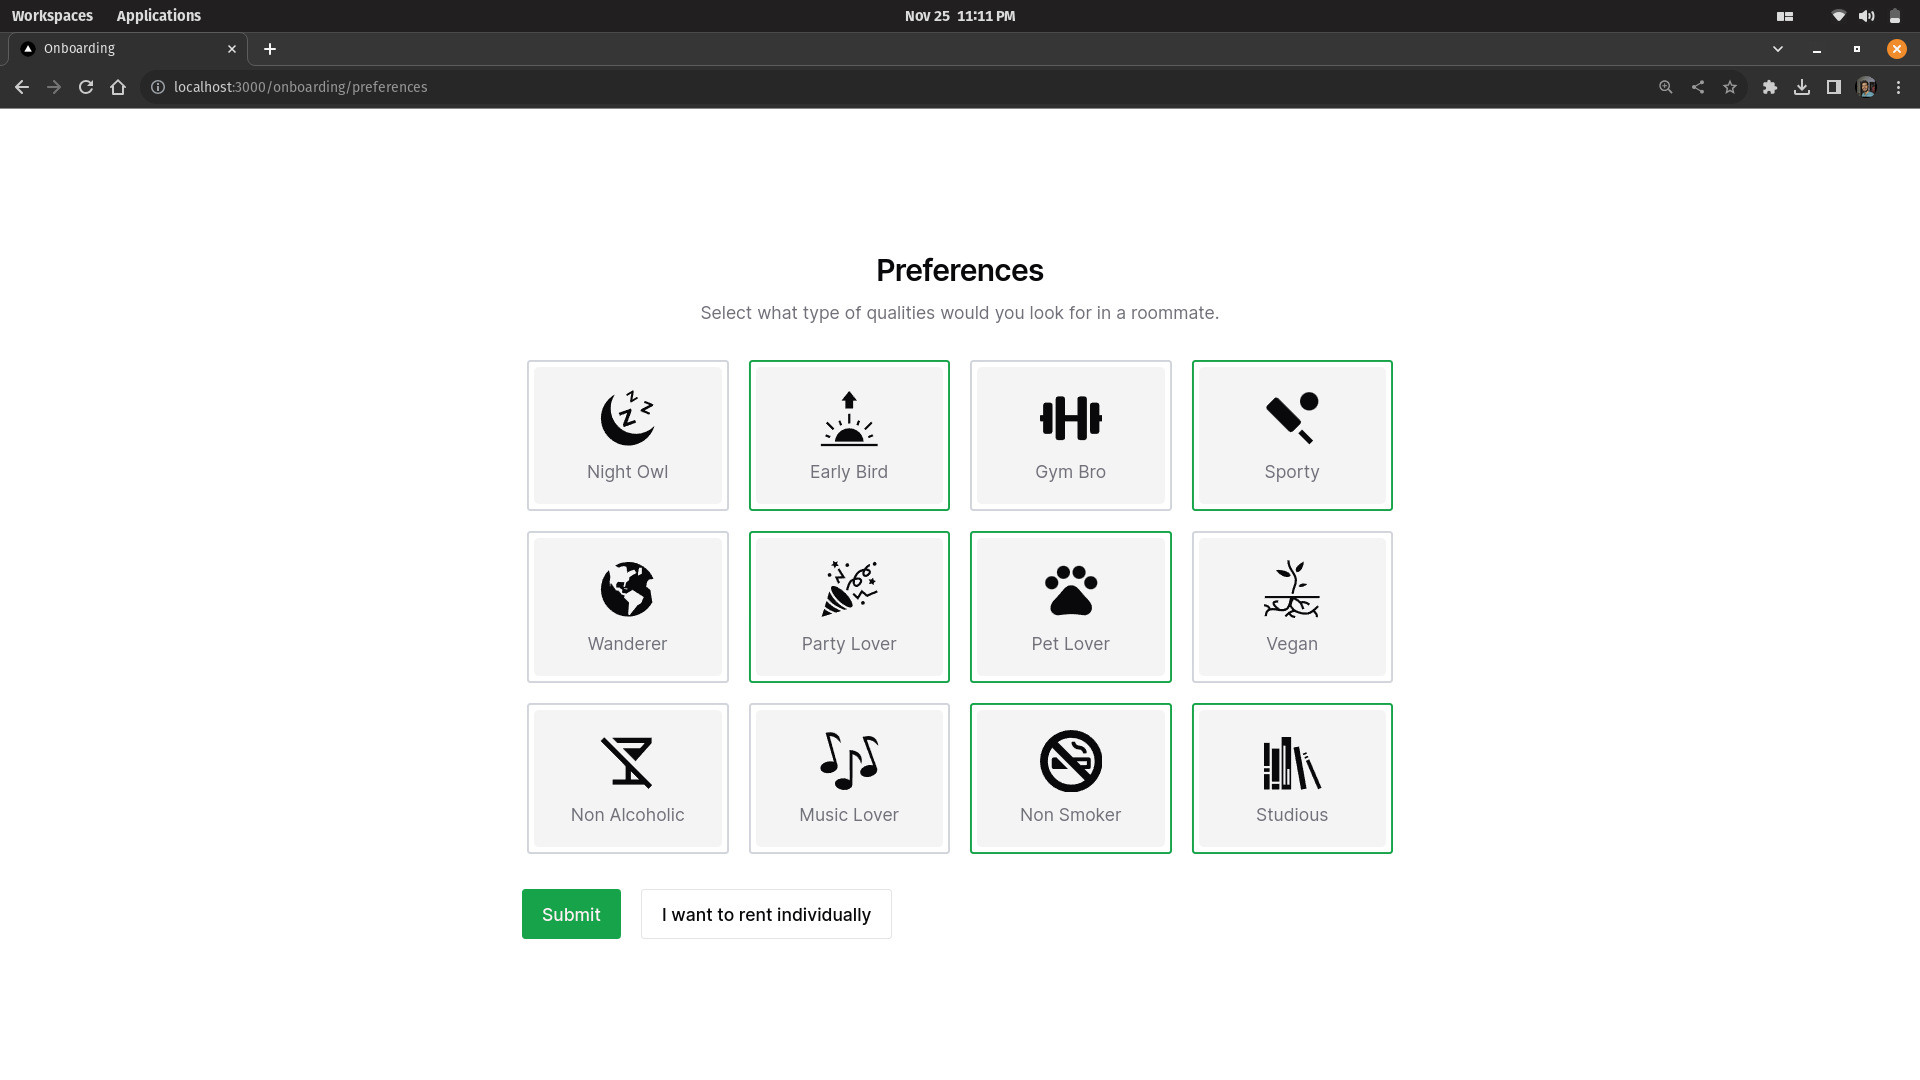
\includegraphics[width=0.8\textwidth]{Images/screenshots/preferences.png}
    \caption{Onboarding Page 2}
\end{figure}
\clearpage

\section{Dashboard}
The dashboard is the main page of the app. It contains various sections that will be discussed in detail in the
below.
\begin{figure}[h]
    \centering
    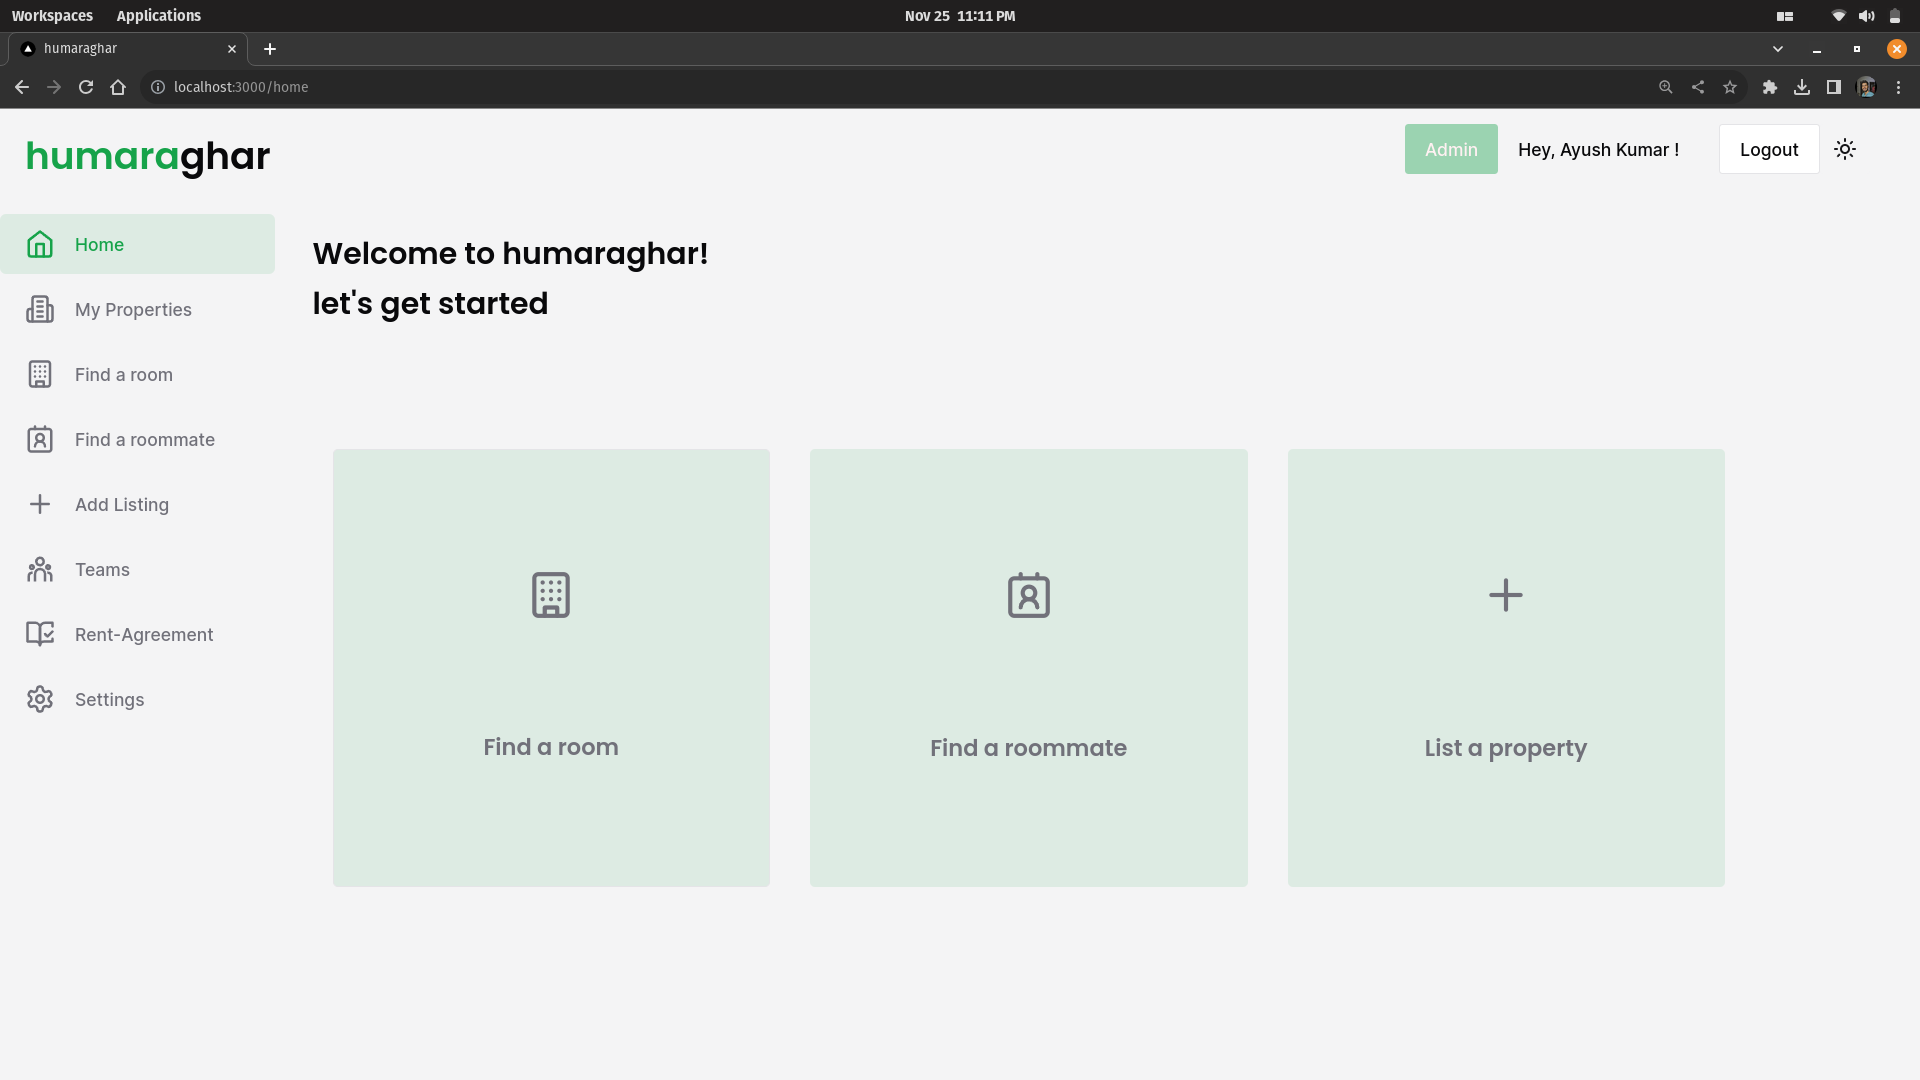
\includegraphics[width=0.8\textwidth]{Images/screenshots/home.png}
    \caption{Dashboard}
\end{figure}

The home page has links to redirect user to main parts of the dashboard catered towards finding a roommate and finding
a room. The user can also view his/her profile by clicking on the profile icon on the top right corner of the page.

\subsection{Find Roommate}
The find roommate page contains a list of all the users that have listing themselves as looking for a shared room, so anymore already having a place to live but looking for a roommate to split
the expenses can find them. Alternatively, you can also team-up among people looking for a room and search for an empty flat together. The user can filter the list based on
location and preferences.


\subsection{Find Room}
The find room page contains a list of all the users that have listing themselves as looking for a roommate, (already having a place to live). The user can filter the list based on
location and preferences again. The rooms which are not shared are also listed here. The user can also view them.

\begin{figure}[h]
    \centering
    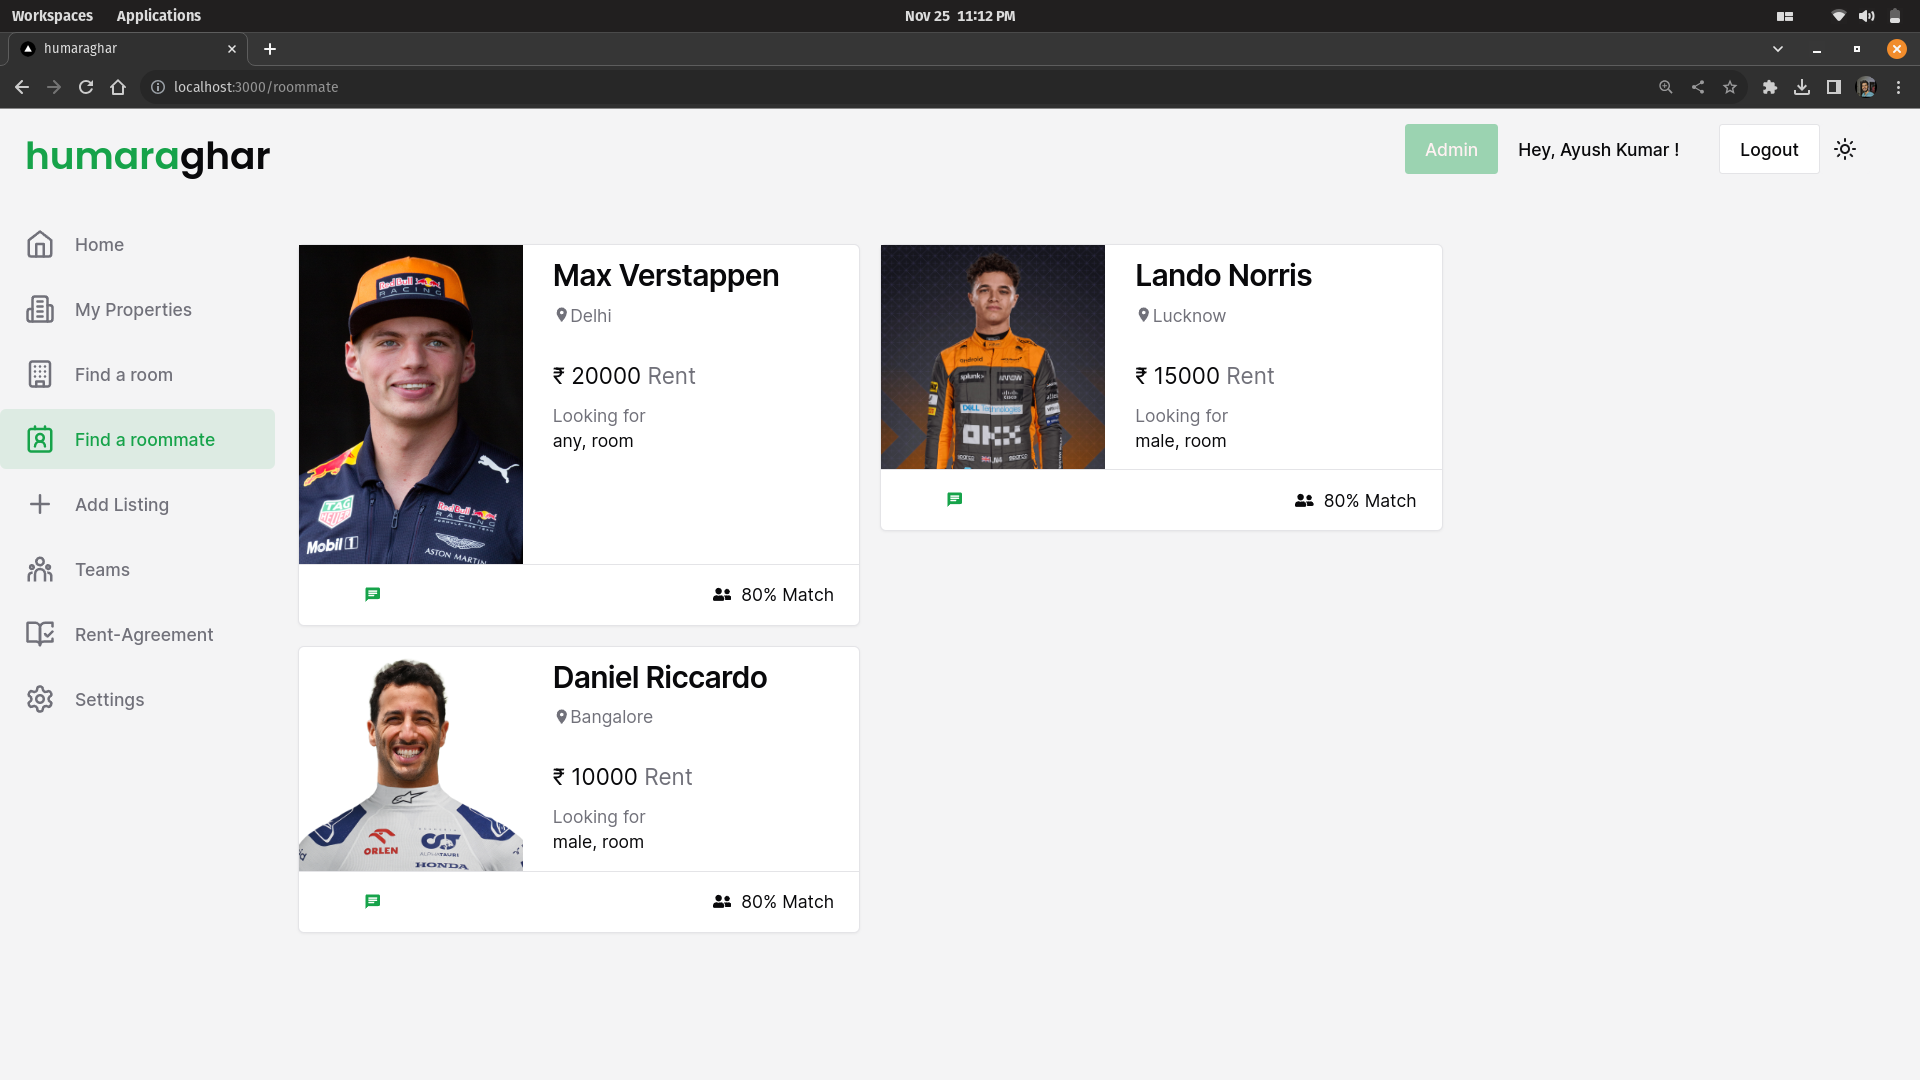
\includegraphics[width=1\textwidth]{Images/screenshots/roommates.png}
    \caption{Find Roommate}
\end{figure}

\begin{figure}[h]
    \centering
    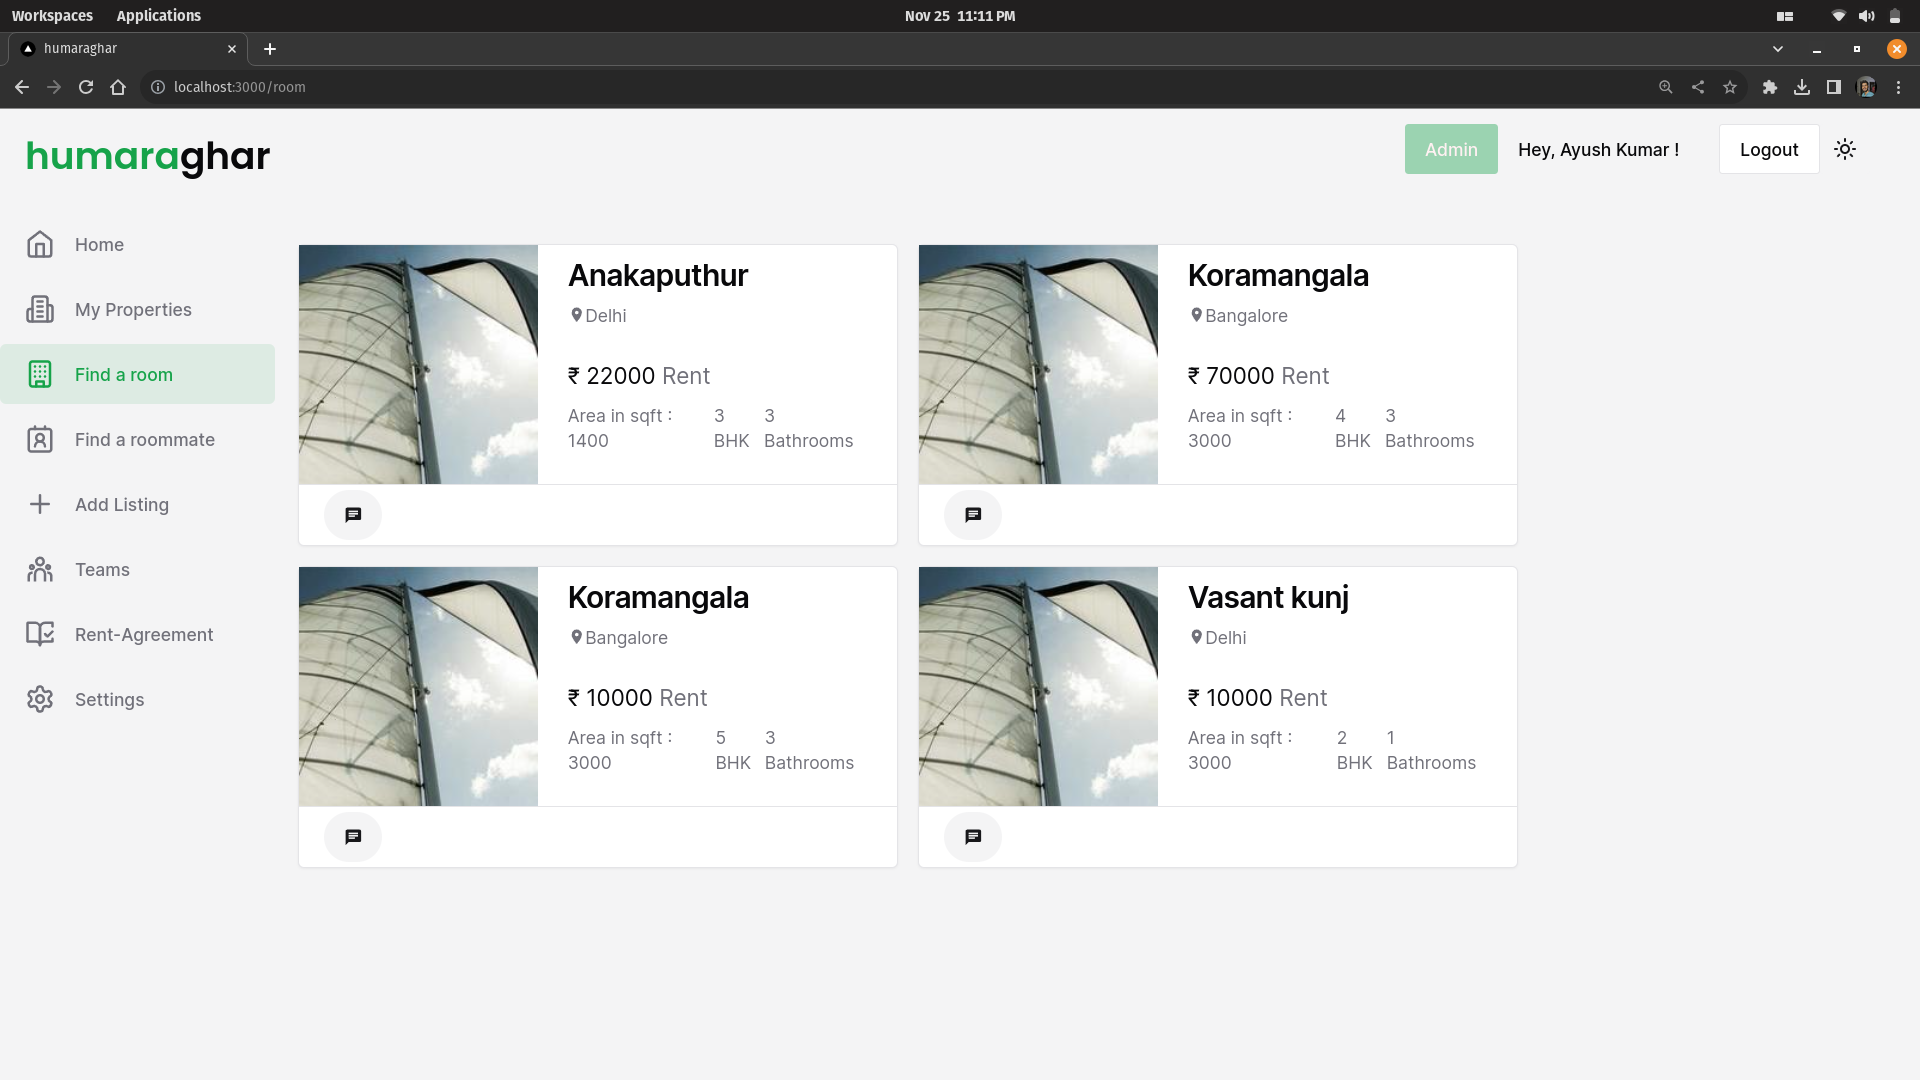
\includegraphics[width=1\textwidth]{Images/screenshots/rooms.png}
    \caption{Find Room}
\end{figure}

\clearpage

The user can either view the detailed description of the room or the roommate by clicking the card. Or he/she can
directly mark themselves interested in the property by clicking the interested button. It will prompt the user to select
if they are interested as a team (if part of any) or individually.

\begin{figure}[h]
    \centering
    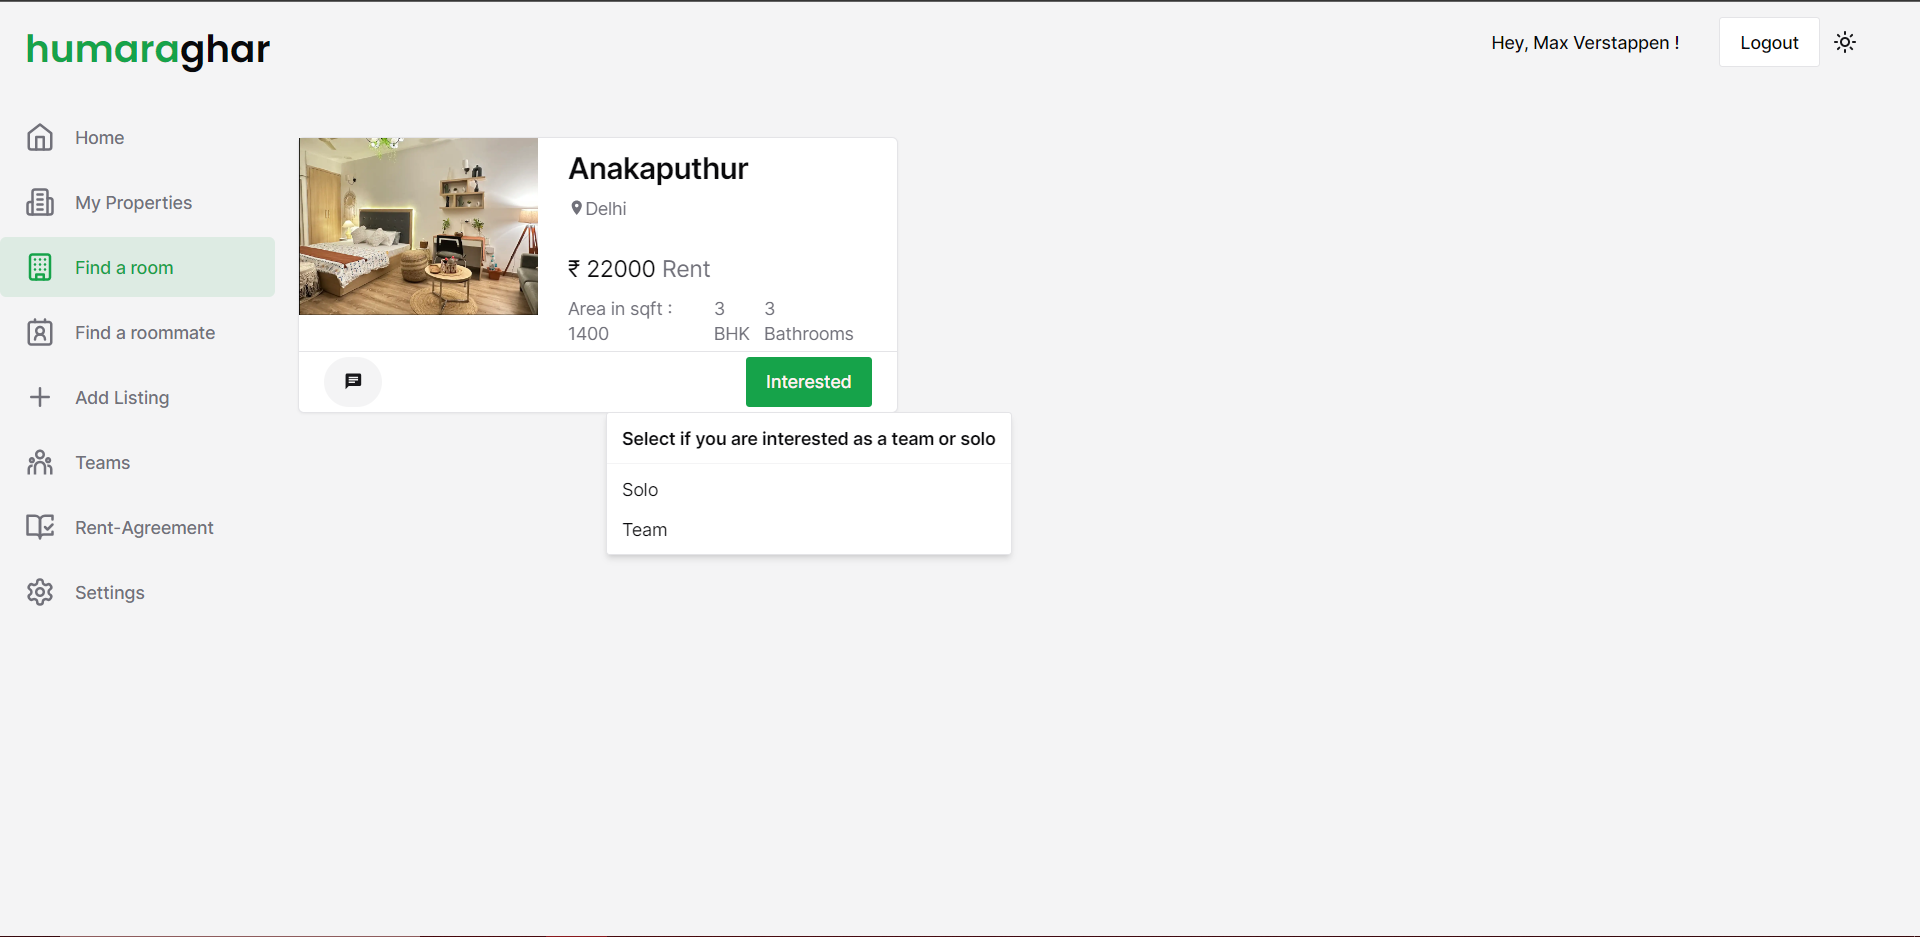
\includegraphics[width=0.8\textwidth]{Images/screenshots/interestedas.PNG}
    \caption{Interested As}
\end{figure}

Clicking as interested would notify the poster and then they can initiate a chat if they are willing to proceed further.
\begin{figure}[h]
    \centering
    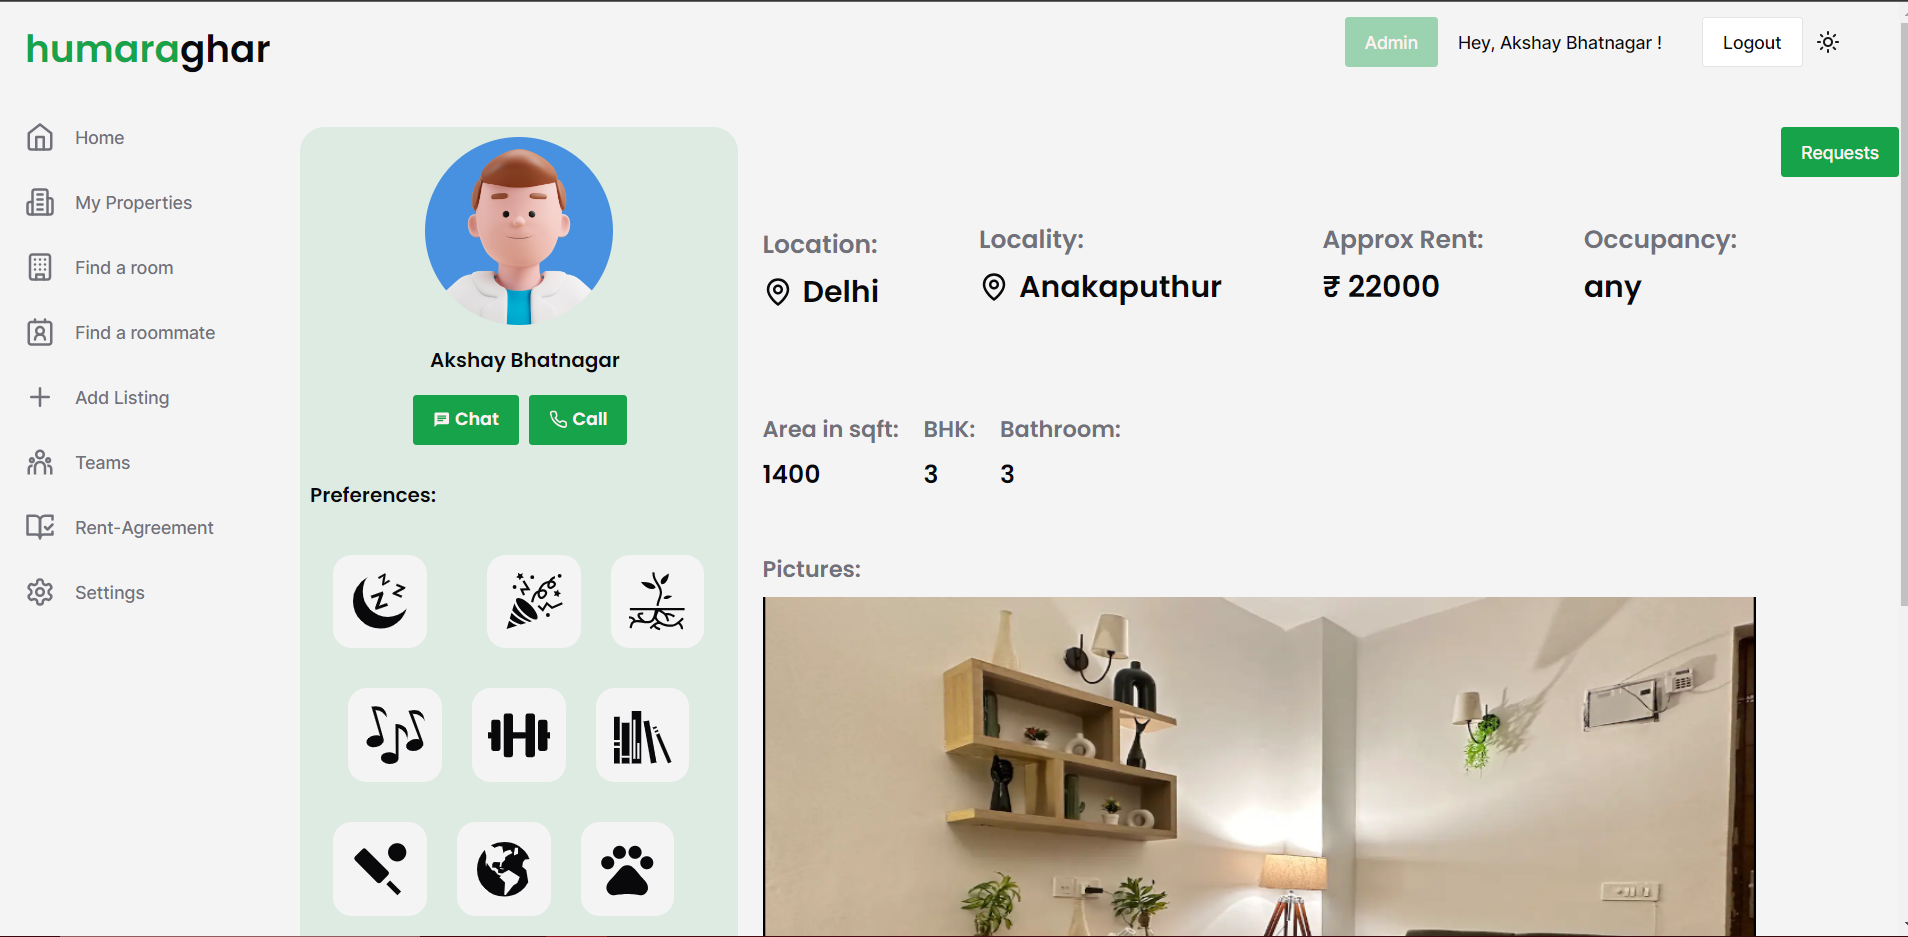
\includegraphics[width=0.8\textwidth]{Images/screenshots/userpage.PNG}
    \caption{Details Page}
\end{figure}
\clearpage

\subsection{Add Listing}
The add listing page is used to add a new listing to the database. The user can add a listing for wanting to share or rent a room.


% Chapter 5

\chapter{Conclusion and Future Work} % Main chapter title

\label{Chapter5} % For referencing  use \ref{Chapter5} 

This semester-long project has culminated in the development of a comprehensive room renting application that caters not only to young professionals seeking shared accommodations but also to families and individuals in pursuit of independent renting options. Originating from our own experiences as young graduates navigating new cities, the application's inception aimed to address the challenges faced by various demographic segments in securing suitable accommodations.\par\medskip

The application's unique proposition lies in its versatility, allowing users to form teams for collaborative housing searches, find compatible roommates, or pursue independent renting without sharing. Leveraging sophisticated machine learning models, the platform aids in suggesting optimal rent prices for listed properties, empowering users with informed decisions.\par\medskip

Throughout the developmental phase, a user-centric approach guided the application's design and functionality. By harnessing Next.js for the frontend and Supabase for the backend, the platform ensures a dynamic, scalable, and intuitive experience for a diverse user base.\par\medskip

This project marks a significant step forward in providing solutions beyond the initial challenges faced by bachelor students entering new cities. The application serves as a comprehensive housing solution, addressing the needs of young professionals, families, and individuals seeking varied housing arrangements.\medskip
\clearpage

Looking ahead, several areas offer opportunities for further development and expansion:
\begin{enumerate}
    \item \textbf{Refinement of Machine Learning Algorithms:} Continuously improve the machine learning models to enhance the accuracy of rent price suggestions and roommate matchmaking, catering to the diverse needs of families and individuals.

    \item \textbf{Geographical and Demographic Expansion:} Expand the application's reach to encompass a broader range of cities and regions, considering the specific requirements of families and individuals seeking independent renting options.

    \item \textbf{Diversified User Experience:} Tailor the user experience to accommodate the distinct preferences of families and individuals, incorporating features like property size specifications, neighborhood suitability, and family-oriented amenities.

    \item \textbf{Adding support for storage units:} Many users don't want to rent complete residential rooms but only someplace to store their belongings. While in western countries the concept of storage rooms are quite popular, there is still a lot of scope for it in India.

    \item \textbf{Feedback-Driven Enhancements:} Implement a robust feedback mechanism to gather insights from families and individuals, enabling iterative improvements and customization based on their experiences and requirements.
\end{enumerate}
\bigskip
In conclusion, this project marks a significant achievement in providing a comprehensive room renting application that caters to the diverse housing needs of families, individuals seeking independent renting, and young professionals. As we move forward, the focus remains on continuous improvement and expansion, driven by user feedback and evolving housing trends.



% Appendix Template

\chapter*{Appendix Title Here}

\label{AppendixX}

\section*{Appendix A: Sample Rent Agreement}
You can find the sample rent agreement \href{http://example.com/agreement}{here}.

\section*{Appendix B: GitHub Repository of our project}
You can find the GitHub repository of our project \href{https://github.com/ayush0402/humara-ghar}{here}.

\section*{Appendix C: GitHub Repository of this LaTeX report}
You can find the GitHub repository of this LaTeX report \href{http://github.com/yourreport}{here}.


\bibliography{Ref}

\end{document}
